\documentclass[%
%draft,
11pt,%
twoside,%
titlepage,%
<<<<<<< Updated upstream
german,%
=======
swissgerman,%
>>>>>>> Stashed changes
headsepline%
]{scrartcl}

\usepackage{lastpage}
\usepackage{amsthm}
\usepackage{amssymb}
\usepackage{geometry}
\usepackage{graphicx}
\usepackage[dvipsnames]{xcolor}
\usepackage[utf8]{inputenc}
<<<<<<< Updated upstream
\usepackage[ngerman]{babel}
=======
\usepackage[swissgerman]{babel}
>>>>>>> Stashed changes
\usepackage{lscape}
\usepackage[framemethod=TikZ]{mdframed}
\usepackage[most]{tcolorbox}
\usepackage{enumerate}
\usepackage{units}
\usepackage{nicefrac}
\usepackage{pgf,tikz}
\usepackage{tikz-3dplot}
\usepackage{tkz-euclide}
\usetikzlibrary{arrows}
\usetikzlibrary{arrows.meta}
\usetikzlibrary{patterns}
\usetikzlibrary{positioning}
\usetikzlibrary{shadows}
<<<<<<< Updated upstream
=======
\usetikzlibrary{quotes, angles}
>>>>>>> Stashed changes
\usepackage{colortbl}
\usepackage{hhline}
\usepackage{multirow}
\usepackage[extendedchars]{grffile}
\usepackage{caption}
\usepackage{multicol,calc}
\usepackage{blindtext}
\usepackage{pdfpages}
\usepackage{hyperref}
\usepackage{framed}

\usepackage{marginnote}
\usepackage{qrcode}
\qrset{height=9ex}

\usepackage{longtable}
\usepackage{listings}
\usepackage{wrapfig}

\usepackage{fontawesome} % Oder FontAwesome, falls du ein Augensymbol aus einer
\newcommand{\faEyeLightGray}{\textcolor{lightgray}{\faEye}} % Custom command for the gray eye icon
<<<<<<< Updated upstream
=======
\newcommand{\faReturnGray}{\textcolor{gray}{\faMailReply}} % Custom command for the gray eye icon
\usepackage{pifont} % weitere Zeichen
>>>>>>> Stashed changes

% package für plots mit dem Befehl axes
\usepackage{pgfplots}



% Command, um Tabellen-Spalten anzupassen
\newcommand{\spaltenheight}{\rule{0mm}{3ex}}
\newcommand{\spaltenwidth}{\rule{3cm}{0mm}}
\newcommand{\spaltensep}{\\[1ex]}
%\arrayrulecolor{darkgreen}
\doublerulesepcolor{white}

% colors
\definecolor{lightyellow}{rgb}{1,1,0.8}
\definecolor{Gray}{gray}{0.9}
\definecolor{lightgray}{rgb}{0.7, 0.7, 0.7}
\definecolor{darkblue}{rgb}{0,0,0.55}
\definecolor{firebrick}{rgb}{0.7,0.13,0.13}
\definecolor{seagreen}{rgb}{0.18,0.55,0.34}
\definecolor{emerald}{HTML}{50C878} % color of Definition
\definecolor{whitesmoke}{HTML}{F5F5F5} % background for environments
\definecolor{myblizzardblue}{HTML}{87CEEB} % color of Satz

% Für Definitionen im Fliesstext
\newcommand{\definition}[1]{\colorbox{emerald}{#1}}
% Für Regeln im Fliesstext
\newcommand{\regel}[1]{\colorbox{myblizzardblue}{#1}}
% Für Merke/Achtungs im Fliesstext
\newcommand{\merke}[1]{\colorbox{firebrick}{#1}}
% Geogebra-Link
\newcommand{\geogebralink}{\href{https://www.geogebra.org/calculator}{\texttt{geogebra.org}}}

% Umgebungen
\theoremstyle{definition}
    \newtheorem{bsp}{Beispiel}[subsection] % Beispiele
    \newtheorem{bem}{Bemerkung}[subsection] % Bemerkungen
\theoremstyle{plain}
    \newtheorem{thm}{Theorem} % Theorem [subsection]
    \newtheorem{satz}{Satz} % Satz [subsection]

% Umgebung lsg mit dynamischer Referenzierung und Label
\newcommand{\concatueb}[1]{ueb:#1}% Definition für concatueb
\newcommand{\concatlsg}[1]{lsg:#1}% Definition für concatlsg

\newcounter{uebcounter}[section]
\renewcommand{\theuebcounter}{\thesection.\arabic{uebcounter}}  % Zählerformat: Abschnitt.Übung

\newenvironment{lsg}[1]{%
<<<<<<< Updated upstream
    \par\noindent\textbf{Notizen zu Übung \ref{\concatueb{#1}}.}%
    \label{\concatlsg{#1}}
=======
    \par\noindent\textbf{Notizen zu Übung \ref{\concatueb{#1}}}\label{\concatlsg{#1}}
    \hfill\hyperref[\concatueb{#1}]{\faReturnGray}\par % Hyperref-Button zurück zur Übung
>>>>>>> Stashed changes
}{%
    \par%
}

\newenvironment{uebenv}[1]{%
    \refstepcounter{uebcounter}
    \par\noindent\textbf{Übung \theuebcounter.}%
    \label{\concatueb{#1}}\hfill\hyperref[\concatlsg{#1}]{\faEyeLightGray}\par
}{%
    \par
}

% Umgebung für Definitionen
\newcounter{deff}[section]\setcounter{deff}{0}
\renewcommand{\thedeff}{\arabic{section}.\arabic{deff}}

\newenvironment{cdef}[1][]{%
    \refstepcounter{deff} 
    \ifstrempty{#1}%
    % if condition (without title)
    {\mdfsetup{%
        frametitle={%
            \tikz[baseline=(current bounding box.east),outer sep=0pt]
            \node[anchor=east,rectangle,fill=emerald]
            {\strut Definition~\thedeff};}
        }%
    % else condition (with title)
    }{\mdfsetup{%
        frametitle={%
            \tikz[baseline=(current bounding box.east),outer sep=0pt]
            \node[anchor=east,rectangle,fill=emerald]
            {\strut Definition~\thedeff:~#1};}%
        }%
    }%
% for both conditions
    \mdfsetup{%
        innertopmargin=10pt,linecolor=emerald,%
        backgroundcolor=whitesmoke,%
        linewidth=2pt,topline=true,%
        frametitleaboveskip=\dimexpr-\ht\strutbox\relax%
    } 
\begin{mdframed}[]\relax}{%
\end{mdframed}}

% Farbig umrahmte Umgebung Satz
\newcounter{satzz}[section]\setcounter{satzz}{0}
\renewcommand{\thesatz}{\arabic{section}.\arabic{satzz}}

\newenvironment{csatz}[1][]{%
    \refstepcounter{satzz}
 
    \ifstrempty{#1}%
    % if condition (without title)
    {\mdfsetup{%
        frametitle={%
            \tikz[baseline=(current bounding box.east),outer sep=0pt]
            \node[anchor=east,rectangle,fill=myblizzardblue]
            {\strut Satz~\thesatz};}
        }%
    % else condition (with title)
    }{\mdfsetup{%
        frametitle={%
            \tikz[baseline=(current bounding box.east),outer sep=0pt]
            \node[anchor=east,rectangle,fill=myblizzardblue]
            {\strut Satz~\thesatz:~#1};}%
        }%
    }%
% for both conditions
    \mdfsetup{%
        innertopmargin=10pt,linecolor=myblizzardblue,%
        backgroundcolor=whitesmoke,%
        linewidth=2pt,topline=true,%
        frametitleaboveskip=\dimexpr-\ht\strutbox\relax%
    }
\begin{mdframed}[]\relax}{%
\end{mdframed}}

% kein Einzug bei neuem Abschnitt
\setlength{\parindent}{0pt} \setlength{\parskip}{1em}
\pagestyle{headings} % gemachte Einstellungen anwenden

\subject{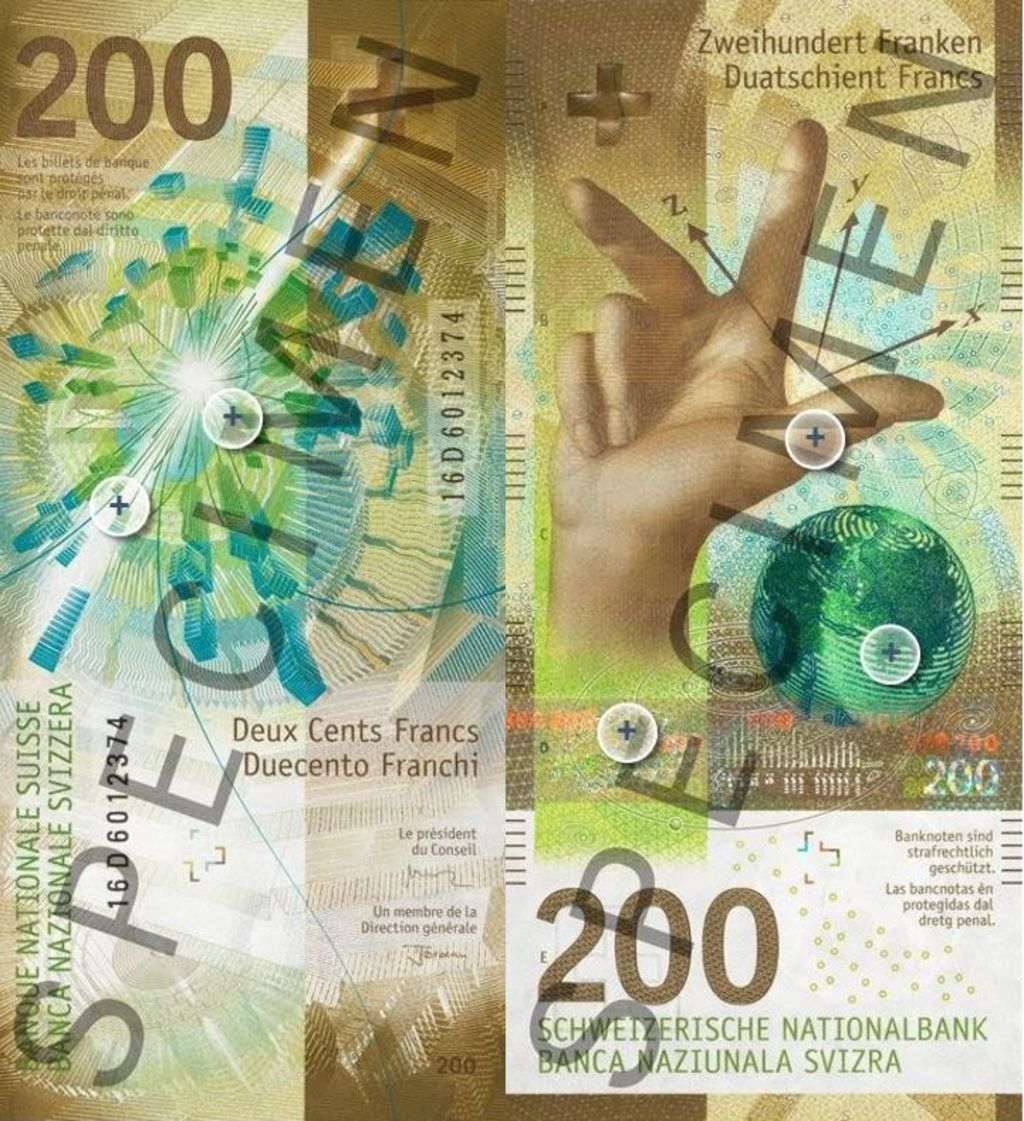
\includegraphics[width=0.618\textwidth]{pictures/200er}}
\title{Vektoren}
\subtitle{Raus in den 3D}
\author{}
\date{}
\lowertitleback{
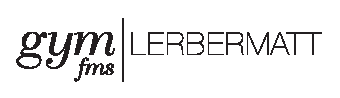
\includegraphics[height=1cm]{pictures/gymfmslerbermattlogo.eps}
\hfill%\copyright%
{\begin{tikzpicture}
  % Draw the rounded rectangle and clip the image to it
  \clip [rounded corners=5mm] (0,0) rectangle (1,1); % Adjust dimensions as needed
  \node at (0.5,0.5) {\includegraphics[width=1cm]{pictures/teacher_me_caricatur.png}}; % Adjust width and center image
\end{tikzpicture}}
}

\begin{document}
\maketitle
\tableofcontents
%\thispagestyle{empty}
\cleardoublepage
%\setcounter{page}{1}

\section{Grundbegriffe}

\subsection{Vektoren}

In unserer Umwelt werden viele Grössen durch Angabe einer reellen Zahl und einer bestimmten Masseinheit beschrieben, z.B. $\unit[10]{s}$, $\unit[4.5]{m^3}$, $\unit[-5]{^\circ C}$, $\unit[100]{g}$. Diese Grössen lassen sich jeweils auf einer Skala (von scalae, lat., Leiter), also durch Punkte auf einer Zahlengeraden, darstellen und heissen deshalb \definition{skalare Grössen}.

Die Geschwindigkeit hingegen ist ein Beispiel für eine Grösse, zu deren vollständiger Festlegung ausser einer Zahl noch die Angabe einer Richtung nötig ist. Auch eine Kraft wird erst durch Angabe von Betrag, Richtung und An\-griffs\-punkt voll\-ständig beschrieben. Derartige Grössen, also Grössen, die durch Festlegung eines Betrags und einer Richtung vollständig bestimmt sind, werden vektorielle Grössen genannt und durch Pfeile (gerichtete Strecken) dargestellt.

Mathematisch werden sie durch Vektoren (vehere, lat., fahren) beschrieben. Man definiert:
\begin{cdef}[Vektor]
Unter einem \textbf{Vektor}
\marginnote{
\qrcode{
https://m.youtube.com/watch?v=WQ2C4uj5QzA}
}
versteht man eine Schar aus sämtlichen untereinander parallelen, gleichgerichteten und gleichlangen Strecken.
\end{cdef}

\begin{figure}[ht]
\begin{center}
\begin{tikzpicture}[line cap=round,line join=round, x=0.4cm,y=0.3cm]
\clip(-4.3,-3.12) rectangle (13.86,6.3);
\draw [thick, -{Latex[length=8pt, width=8pt]}] (-2,1) -- (0,4);
\draw [thick, -{Latex[length=8pt, width=8pt]}] (-1,-1) -- (1,2);
\draw [thick, -{Latex[length=8pt, width=8pt]}] (5,3) -- (7,6);
\draw [thick, -{Latex[length=8pt, width=8pt]}] (7,-2) -- (9,1);
\draw [thick, -{Latex[length=8pt, width=8pt]}] (8,1) -- (10,4);
\draw [thick, -{Latex[length=8pt, width=8pt]}] (10,-1) -- (12,2);
\draw [thick, -{Latex[length=8pt, width=8pt]}] (2,-2) -- (4,1);
\end{tikzpicture}
\end{center}
\caption{Vektor-Schar}
\end{figure}

Damit ist ein Vektor eine unendliche Menge von gerichteten Strecken: Von jedem Punkt der Ebene bzw. des Raumes geht genau eine solche Strecke aus, wobei alle diese Strecken untereinander parallel und gleichgerichtet sind und die gleiche Länge haben.

In Abbildungen wird ein Vektor als eine Strecke mit Pfeilspitze gezeichnet, d.h. man zeichnet nicht die ganze Schar von gerichteten Strecken, die den Vektor darstellen, sondern nur eine dieser Strecken, einen sogenannten \definition{Repräsentanten}.

\begin{figure}
\begin{center}
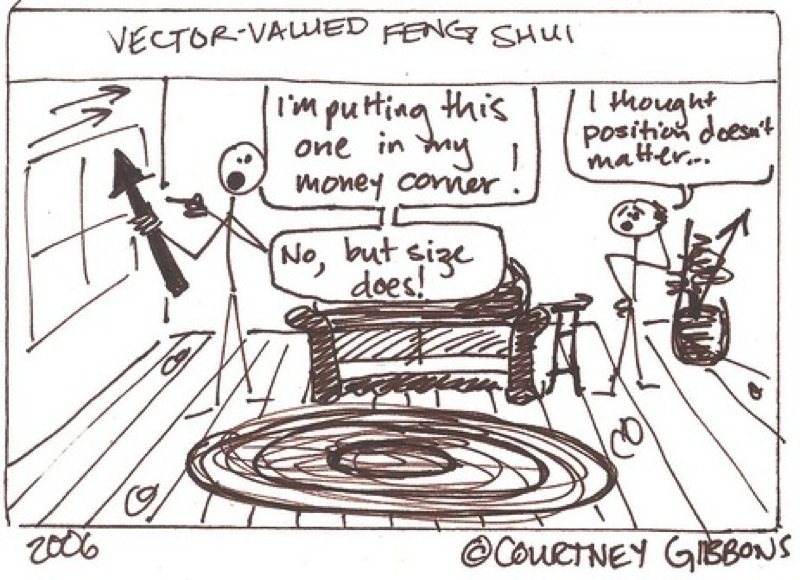
\includegraphics[width=0.618\textwidth]{pictures/repraesentant}
\end{center}
\caption{Repräsentant}
\end{figure}

\begin{bem}
Eine ähnliche Situation liegt bei den Zahlen vor: Vergleiche die Brüche
$$\frac{1}{4}, \frac{2}{8}, \frac{-3}{-12}, \frac{90}{360}, \dots$$
die durch Kürzen und Erweitern ineinander übergeführt werden können. Sie sind alle dem gleichen Punkt auf der Zahlengeraden zugeordnet. Jeder derartige Bruch kann als Repräsentant zur Angabe der rationalen Zahl $0.25$ herangezogen werden.
\end{bem}

Die Vektoren werden mit $\vec{a}, \vec{b}, \vec{c}, \vec{v}, \vec{w}, \dots$ oder mit $\vec{AB}, \vec{PQ},\dots$, wobei der erste Buchstabe den Anfangspunkt, der zweite den Endpunkt angibt, bezeichnet. Der darüber gesetzte Pfeil deutet an, dass es sich um einen Vektor und nicht etwa \glqq nur\grqq\ um einen Skalar handelt.

Die \definition{Länge} oder Betrag eines Vektors schreibt man in der Form $|\vec{v}|$ oder auch kurz $v$ bzw. $|\vec{PQ}|$; für die Richtung verwendet man kein besonderes Zeichen. Man gibt zum Beispiel in der Ebene die \definition{Richtung} als Winkel zwischen Vektor und positiver $x$-Achse an.

\begin{figure}[ht]
\begin{center}
\definecolor{qqwuqq}{rgb}{0,0.39,0}
\definecolor{cqcqcq}{rgb}{0.75,0.75,0.75}
\scalebox{1.2}{
\begin{tikzpicture}[line cap=round,line join=round, x=0.5cm,y=0.5cm]
\draw [color=cqcqcq,dash pattern=on 2pt off 2pt, xstep=0.5cm,ystep=0.5cm] (-3.5,-2.6) grid (6.8,3.5);
\draw[->,color=black] (-4.04,0) -- (7.94,0);
\foreach \x in {-4,-3,-2,-1,1,2,3,4,5,6,7}
\draw[shift={(\x,0)},color=black] (0pt,2pt) -- (0pt,-2pt) node[below] {\footnotesize $\x$};
\draw[color=black] (7.6,0.08) node [anchor=south west] {$x$};
\draw[->,color=black] (0,-2.98) -- (0,4.34);
\foreach \y in {-2,-1,1,2,3,4}
\draw[shift={(0,\y)},color=black] (2pt,0pt) -- (-2pt,0pt) node[left] {\footnotesize $\y$};
\draw[color=black] (0.1,3.94) node [anchor=west] {$y$};
\draw[color=black] (0pt,-10pt) node[right] {\footnotesize $0$};
\clip(-4.04,-2.98) rectangle (7.94,4.34);
\draw [shift={(5,1)},color=qqwuqq,fill=qqwuqq,fill opacity=0.05] (0,0) -- (0:1) arc (0:153.43:1) -- cycle;
\draw [thick, -{Latex[length=8pt, width=8pt]}] (5,1) -- (1,3);
\draw[color=black] (3.14,2.4) node {$\vec{v}$};
\draw[color=qqwuqq] (5.1,1.4) node {$\varphi$};
\end{tikzpicture}
}
\end{center}
\caption{Betrag und Richtung}\label{vecdef}
\end{figure}

\begin{uebenv}{laengeundrichtung}
Bestimme Länge und Richtung von $\vec{v}$ aus Abbildung \ref{vecdef} auf Seite \pageref{vecdef}.
\end{uebenv}

Entscheidend für die Einführung von Vektoren ist die Tatsache, dass man für sie Rechengesetze angeben und infolgedessen mit ihnen --- ähnlich wie in der Arithmetik mit Zahlen oder in der Algebra mit Buchstaben --- rechnen kann.

\begin{bem}
Um die algebraische Struktur zu vervollständigen, auf denen die einzuführenden Rechengesetze gelten, lässt man Strecken der Länge Null zu. Obwohl für solche Strecken keine Richtung definiert ist, ist es zweckmässig, diese als \definition{Nullvektor} $\vec{0}$ zu bezeichnen. Der Nullvektor hat den Betrag $0$ und keine Richtung.
\end{bem}

Oft ist es beim Rechnen mit Vektoren hilfreich, die Aufgabenstellung geometrisch zu interpretieren.

\begin{bem}
Ein Vektor kann geometrisch als Translation aufgefasst werden, der den Anfangspunkt in den Endpunkt abbildet.
\end{bem}

Heute gilt die Vektorrechnung in der Mathematik und ihren Anwendungen in den Naturwissenschaften als ein unentbehrliches Hilfsmittel. Als herausragendes Beispiel seien hier nur die vier Maxwell'schen Vektorgleichungen erwähnt, die für die Elektrodynamik ein ähnliches Axiomensystem wie die Newton'schen Grundgleichungen für die Mechanik bilden (\textsc{James Clerk Maxwell}, 1831-1879).

\begin{align*}
\nabla\cdot\vec{E} &= \frac{\rho}{\epsilon_0}\tag{Ladung ist Quelle des elektrischen Feldes}\\
\nabla\cdot\vec{B} &= 0\tag{Es gibt keine magnetischen Monopole}\\
\nabla\times\vec{E} &= -\frac{\partial \vec{B}}{\partial t}\tag{\"Anderung mag. Feld führt zu el. Wirbelfeld}\\
\nabla\times\vec{B} &= \mu_0\vec{j}+\mu_0\epsilon_0\frac{\partial\vec{E}}{\partial t}\tag{el. Strom führt zu mag. Wirbelfeld}
\end{align*}

Wer sich bereits etwas mit Vektoren auskennt, für den sei hier am Rande der QR-Code zum Video \emph{Vektoren in 10 Minuten} angedacht.
\marginnote{
\qrcode{
https://www.youtube.com/watch?v=tw6_eu___Sk}
}

\begin{uebenv}{betragundrichtung}
Berechne die Beträge und die Richtungen (Winkel $\vec{a}rphi$ zwischen Pfeil und $x$-Achse) der eingezeichneten Vektoren.
\begin{center}
\definecolor{cqcqcq}{rgb}{0.75,0.75,0.75}
\begin{tikzpicture}[line cap=round,line join=round, x=0.45cm,y=0.45cm]
\draw [color=cqcqcq,dash pattern=on 2pt off 2pt, xstep=0.45cm,ystep=0.45cm] (-7.56,-5.2) grid (7.4,4.5);
\draw[->,color=black] (-7.56,0) -- (8.16,0);
\foreach \x in {-7,-6,-5,-4,-3,-2,-1,1,2,3,4,5,6,7,8}
\draw[shift={(\x,0)},color=black] (0pt,2pt) -- (0pt,-2pt) node[below] {\footnotesize $\x$};
\draw[color=black] (7.82,0.08) node [anchor=south west] { x};
\draw[->,color=black] (0,-5.56) -- (0,5.54);
\foreach \y in {-5,-4,-3,-2,-1,1,2,3,4,5}
\draw[shift={(0,\y)},color=black] (2pt,0pt) -- (-2pt,0pt) node[left] {\footnotesize $\y$};
\draw[color=black] (0.1,5.14) node [anchor=west] { y};
\clip(-7.56,-5.56) rectangle (8.16,5.54);
\draw [thick, -{Latex[length=8pt, width=8pt]}] (-1,4) -- (-7,2);
\draw [thick, -{Latex[length=8pt, width=8pt]}] (-5,-4) -- (-3,1);
\draw [thick, -{Latex[length=8pt, width=8pt]}] (1,1) -- (6,2);
\draw [thick, -{Latex[length=8pt, width=8pt]}] (2,-2) -- (4,-2);
\draw [thick, -{Latex[length=8pt, width=8pt]}] (6.5,-5) -- (-2,-3);
\draw[color=black] (-4.1,3.5) node {$\vec{u}$};
\draw[color=black] (-4.4,-1.32) node {$\vec{v}$};
\draw[color=black] (3.26,1.9) node {$\vec{w}$};
\draw[color=black] (2.96,-1.4) node {$\vec{b}$};
\draw[color=black] (2.5,-3.5) node {$\vec{a}$};
\end{tikzpicture}
\end{center}
\end{uebenv}

\clearpage

\subsection{Notizen zu den Übungen}

\begin{lsg}{laengeundrichtung}
    Die Länge ist nach Pythagoras $\sqrt{4^2+2^2}=\sqrt{20}=2\sqrt{5}\approx4.5$. Für den Winkel brauchen wir $\tan(\varphi)=\frac{2}{4}$ und erhalten $\varphi=\arctan(\frac{1}{2})\approx27^\circ$
\end{lsg}
\begin{lsg}{betragundrichtung}
    \begin{enumerate}[a)]
        \item Länge $\sqrt{8.5^2+2^2}\approx8.7$, der Winkel ist $\varphi=\arctan(\frac{2}{8.5})\approx13^\circ$
        \item Länge $2$ und Winkel $0^\circ$
        \item $u=\sqrt{6^2+2^2}=\sqrt{40}=2\sqrt{10}$ und Winkel $\varphi=\arctan(\frac{1}{3})+180^\circ$
        \item $v=\sqrt{2^2+5^2}$ und $\varphi=\arctan(\frac{5}{2})$
        \item $w=\sqrt{26}$ und $\varphi=\arctan(\frac{1}{5})$
    \end{enumerate}
\end{lsg}

\clearpage

\section{Grundoperationen mit Vektoren}

Wir wollen uns zuerst mit der geometrischen Interpretation der Grundoperationen auseinandersetzen. Die algebraische Umsetzung ist dann \glqq einfach\grqq\ durch Angabe von Definitionen zu erledigen, die die Geometrie repräsentieren.

\subsection{Gegenvektor}

\begin{cdef}[Gegenvektor]
Der Vektor, der zwar den gleichen Betrag, aber die entgegengesetzte Richtung wie $\vec{v}$ hat, wird mit $-\vec{v}$ bezeichnet und heisst Gegenvektor von $\vec{v}$.
\end{cdef}

\begin{figure}[ht]
\begin{center}
\definecolor{cqcqcq}{rgb}{0.75,0.75,0.75}
\scalebox{1}{
\begin{tikzpicture}[line cap=round,line join=round, x=0.6cm,y=0.6cm]
\draw [color=lightgray,dash pattern=on 3pt off 3pt, xstep=0.3cm,ystep=0.3cm] (-4.3,1.16) grid (6.72,6.3);
\clip(-4.3,1.16) rectangle (6.72,6.3);
\draw [thick, -{Latex[length=8pt, width=8pt]}] (3,5) -- (-3,3);
\draw [thick, -{Latex[length=8pt, width=8pt]}] (-1,2) -- (5,4);
\end{tikzpicture}
}
\end{center}
\caption{Vektor und Gegenvektor}
\end{figure}

\subsection{S-Multiplikation}

Analog definiert man die Multiplikation eines Vektors mit einem Skalar.

\begin{cdef}[S-Multiplikation]
Für $t\in\mathbb{R}$ ist $t\cdot\vec{a}$ ein Vektor mit dem $|t|$-fachen Betrag von $\vec{a}$:
$$|t\vec{a}|=|t|\vec{a}.$$
Diese Operation nennt man kurz S-Multiplikation.
\begin{itemize}
\item Falls $t>0$ ist, hat $t\vec{a}$ dieselbe Richtung wie $\vec{a}$,
\item Falls $t<0$ ist, hat $t\vec{a}$ die entgegengesetzte Richtung von $\vec{a}$,
\item falls $t=0$ ist, ist $t\vec{a}$ der Nullvektor.
\end{itemize}
\end{cdef}

\begin{figure}[ht]
\begin{center}
\begin{tikzpicture}[line cap=round,line join=round, x=0.618cm,y=0.618cm]
\clip(-0.18,-1.04) rectangle (8.9,4.24);
\draw [thick, -{Latex[length=8pt, width=8pt]}] (0.5,0.5) -- (1.5,2.5);
\draw [thick, -{Latex[length=8pt, width=8pt]}] (2,-0.5) -- (4,3.5);
\draw [thick, -{Latex[length=8pt, width=8pt]}] (6,3) -- (4.5,0);
\draw[color=black] (0.6,1.5) node {$\vec{v}$};
\draw[color=black] (2.6,1.68) node {$2\vec{v}$};
\draw[color=black] (4.3,1.5) node {$-1.5\vec{v}$};
\fill [color=black] (7.5,1.5) circle (1.5pt);
\draw[color=black] (7.66,1.9) node {$\vec{0}$};
\end{tikzpicture}
\end{center}
\caption{S-Multiplikation}
\end{figure}

Umgekehrt gilt
\begin{bem}
Sind zwei Vektoren $\vec{v}$ und $\vec{w}$ zu ein und derselben Geraden parallel, so ist $\vec{w}$ ein Vielfaches von $\vec{v}$, d.h.
$$\vec{w}=t\vec{v}$$
\end{bem}

\begin{cdef}[kollinear]
Zwei Vektoren $\vec{v}$ und $\vec{w}$, für die $$\vec{w}=t\vec{v}$$ gilt, heissen kollinear.
\end{cdef}

\begin{cdef}[Einheitsvektor]
Ein Vektor mit Betrag $1$ heisst Einheitsvektor.
\end{cdef}

Insbesondere bezeichnen wir die Einheitsvektoren in $x$- bzw. $y$-Richtung mit $\vec{e}_x$ bzw. $\vec{e}_y$.

\subsection{Addition und Subtraktion}

Man legt fest
\begin{cdef}[Addition]
Die \textbf{Summe}
\marginnote{
\qrcode{
https://m.youtube.com/watch?v=eiIF6NDyYqU}
}
$\vec{v}+\vec{w}$ zweier Vektoren $\vec{v}$ und $\vec{w}$ ist der Vektor $\vec{u}$, den man durch \glqq Aneinandersetzen\grqq\ von $\vec{v}$ und $\vec{w}$ erhält.
\end{cdef}

\begin{figure}[ht]
\begin{center}
\begin{tikzpicture}[line cap=round,line join=round, x=0.5cm,y=0.4cm]
\clip(-4.3,-1.26) rectangle (7.06,6.3);
\draw [thick, -{Latex[length=8pt, width=8pt]}] (-3,0) -- (3,0);
\draw [thick, -{Latex[length=8pt, width=8pt]}] (3,0) -- (6,5);
\draw [thick, -{Latex[length=8pt, width=8pt]} , color=firebrick] (-3,0) -- (6,5);
\fill [color=darkblue] (-3,0) circle (1.5pt);
\draw[color=darkblue] (-3.5,0.18) node {$A$};
\fill [color=darkblue] (3,0) circle (1.5pt);
\draw[color=darkblue] (3.5,-0.08) node {$B$};
\draw[color=black] (-0.02,-0.5) node {$\vec{v}$};
\fill [color=darkblue] (6,5) circle (1.5pt);
\draw[color=darkblue] (6.2,5.7) node {$C$};
\draw[color=black] (4.9,2.32) node {$\vec{w}$};
\draw[color=firebrick] (0.1,3.1) node {$\vec{u}=\vec{v}+\vec{w}$};
\end{tikzpicture}
\end{center}
\caption{Vektoraddition}
\end{figure}

Der Summenvektor $\vec{u}=\vec{v}+\vec{w}$ hat seinen Anfangspunkt im Anfangspunkt des ersten Summanden und seinen Endpunkt im Endpunkt des zweiten Summanden:
$$\vec{AB}+\vec{BC}=\vec{AC}$$

\begin{bem}
$\vec{u}=\vec{v}+\vec{w}$ entspricht der Diagonalen des von $\vec{v}$ und $\vec{w}$ aufgespannten Parallelogramms.
\end{bem}

\begin{cdef}[Subtraktion]
Die Subtraktion wird auf die Addition zurückgeführt:
$$\vec{u}=\vec{v}-\vec{w}=\vec{v}+(-\vec{w})$$
\end{cdef}

Man subtrahiert den Vektor $\vec{w}$ vom Vektor $\vec{v}$, indem
man zu $\vec{v}$ den Gegenvektor von $\vec{w}$ addiert. Aus $\vec{u}=\vec{v}-\vec{w}$ ergibt sich sofort $\vec{u}+\vec{w}=\vec{v}$. Um die Differenz $\vec{v}-\vec{w}$ zu erhalten, genügt es, die Vektoren $\vec{v}$ und $\vec{w}$ an einem Punkt $P$ anzutragen und den Vektor aufzusuchen, der vom Endpunkt des Vektors $\vec{w}$ zum Endpunkt des Vektors $\vec{v}$ reicht.

\begin{figure}[ht]
\begin{center}
\begin{tikzpicture}[line cap=round,line join=round, x=0.8cm,y=0.8cm]
\clip(-4.26,-0.76) rectangle (3.7,4.52);
\draw [thick, -{Latex[length=8pt, width=8pt]}] (-3,1.5) -- (-2,3.5);
\draw [thick, -{Latex[length=8pt, width=8pt]}] (-4,0.5) -- (-1,0.02);
\draw [thick, -{Latex[length=8pt, width=8pt]}] (0,1) -- (1,3);
\draw [thick, -{Latex[length=8pt, width=8pt]}] (0,1) -- (3,0.5);
\draw [thick, -{Latex[length=8pt, width=8pt]}, color=firebrick] (3,0.5) -- (1,3);
\draw[color=black] (-2.82,2.66) node {$\vec{v}$};
\draw[color=black] (-2.58,0.62) node {$\vec{w}$};
\draw[color=black] (0.2,2.04) node {$\vec{v}$};
\draw[color=black] (1.26,0.58) node {$\vec{w}$};
\draw[color=firebrick] (2.14,2.06) node {$\vec{u}$};
\end{tikzpicture}
\end{center}
\caption{Subtraktion von Vektoren}
\end{figure}

\begin{bem}
Mit dieser Definition erzielt man auch eine Übereinstimmung mit dem in der Physik experimentell nachgewiesenen \glqq Kräfteparallelogramm\grqq. Wenn an einem Körper die Kräfte $\vec{F}_1$ und $\vec{F}_2$ am gleichen Punkt angreifen, dann können sie durch die \definition{resultierende} Kraft $\vec{F}_R$ ersetzt werden, welche die vektorielle Summe der angreifenden Kräfte ist:
$$\vec{F}_R = \vec{F}_1 + \vec{F}_2$$

\begin{figure}[ht]
\begin{center}
\scalebox{0.8}{
\begin{tikzpicture}[line cap=round,line join=round, x=0.7cm,y=0.8cm]
\clip(-4.26,-1.3) rectangle (5.58,4.52);
\draw [thick, -{Latex[length=8pt, width=8pt]}] (-3,0) -- (3,0);
\draw [thick, -{Latex[length=8pt, width=8pt]}] (-3,0) -- (-1,4);
\draw [dash pattern=on 5pt off 5pt] (-1,4)-- (5,4);
\draw [dash pattern=on 5pt off 5pt] (5,4)-- (3,0);
\draw [thick, -{Latex[length=8pt, width=8pt]}] (-3,0) -- (5,4);
\draw [rotate around={-64.87:(-2.92,0.09)},fill=black,fill opacity=0.15] (-2.92,0.09) ellipse (1.15cm and 0.73cm);
\draw[color=black] (0.04,-0.26) node {$\vec{F}_1$};
\draw[color=black] (-2.3,2.38) node {$\vec{F}_2$};
\draw[color=black] (1,2.5) node {$\vec{F}_R$};
\end{tikzpicture}
}
\end{center}
\caption{Kräfteparallelogramm}
\end{figure}
\end{bem}

\begin{uebenv}{pfeilchenzeichnen}
Gegeben seien die Vektoren $\vec{u},\vec{v}$ und $\vec{w}$.

\begin{center}
\begin{tikzpicture}[line cap=round,line join=round, x=1cm,y=1cm]
\draw [color=lightgray,dash pattern=on 2pt off 2pt, xstep=0.5cm,ystep=0.5cm] (-4.26,0.16) grid (2.4,4.4);
\clip(-4.26,0.16) rectangle (2.58,4.52);
\draw [thick, -{Latex[length=8pt, width=8pt]}] (-3.5,4) -- (-1.5,3);
\draw [thick, -{Latex[length=8pt, width=8pt]}] (-4,1.5) -- (-1,1.5);
\draw [thick, -{Latex[length=8pt, width=8pt]}] (0,1) -- (2,3);
\draw[color=black] (-2.42,3.72) node {$\vec{u}$};
\draw[color=black] (-2.44,1.72) node {$\vec{v}$};
\draw[color=black] (0.72,2.24) node {$\vec{w}$};
\end{tikzpicture}
\end{center}
Skizziere:
\begin{enumerate}[a)]
\item $\vec{r}=\vec{u}-\vec{v}$
\item $\vec{a}=\vec{u}-2\vec{v}+0.5\vec{w}$
\item $\vec{b}=3\vec{u}-1.5\vec{v}+2\vec{w}$
\end{enumerate}
\end{uebenv}

\begin{uebenv}{aareschwumm}
Ein
\marginnote{
\qrcode{
https://m.youtube.com/watch?v=yrQB3sX_HOM}
}
Schwimmer ($v_s = \unitfrac[1.5]{m}{s}$) will einen $\unit[20]{m}$ breiten Fluss ($v_F = \unitfrac[1.2]{m}{s}$)
\begin{enumerate}[a)]
\item auf kürzestem Wege,
\item in kürzester Zeit
\end{enumerate}
überqueren. Berechne jeweils die Dauer und zusätzlich den Vorhaltewinkel und die Abdrift.
\end{uebenv}

\begin{uebenv}{beweismittellinie}
Zeige, dass die Mittellinie eines Dreiecks halb so
lang wie die Grundlinie und parallel zu dieser ist.
\end{uebenv}

\begin{uebenv}{halbiertediagonalen}
Halbieren
\marginnote{
\qrcode{
https://m.youtube.com/watch?v=mbfcd-n5saI}
}
sich in einem Viereck die Diagonalen, so ist es ein Parallelogramm?!

Und, hat man ein Parallelogramm, so halbieren sich die Diagonalen.
\end{uebenv}

Ein ausserordentlich nützlicher Satz lässt sich über nicht kollineare Vektoren formulieren:

\begin{csatz}[Satz zur linearen Abhängigkeit]\label{csatzlinunabh}
Sind $\vec{v}$ und $\vec{w}$ nicht kollinear und $$\lambda\vec{v}+\mu\vec{w}=\vec{0},$$ dann muss $\lambda=0$ \emph{und} $\mu=0$ sein.
\end{csatz}

\begin{proof}[Beweis]
Es seien $\vec{v}$ und $\vec{w}$ nicht kollinear abhängig und $\lambda\vec{v}+\mu\vec{w}=\vec{0}$. OEdA $\lambda\neq0$, dann gälte $\vec{v}=-\frac{\mu}{\lambda}\vec{w}$. Dies ist ein Widerspruch zur Annahme, dass $\vec{v}$ und $\vec{w}$ nicht kollinear sind. Analog geht man für $\mu$ vor.
\end{proof}

Die lineare Unabhängigkeit zweier Vektoren $\vec{v}$ und $\vec{w}$ lässt sich geometrisch veranschaulichen, wenn man die Diagonale des von $\lambda\vec{v}$ und $\mu\vec{w}$ aufgespannten Parallelogramms betrachtet. Diese Diagonale entspricht nur dann dem Nullvektor, wenn $\lambda=0$ und zugleich $\mu=0$ wird.

\begin{cdef}[lineare Unabhängigkeit]
Man nennt zwei nicht kollineare Vektoren linear unabhängig.
\end{cdef}

\clearpage

\subsection{Notizen zu den Übungen}

\begin{lsg}{pfeilchenzeichnen}

\begin{tikzpicture}[line cap=round,line join=round,x=1cm,y=1cm]
\draw [color=lightgray,dash pattern=on 2pt off 2pt, xstep=0.5cm,ystep=0.5cm] (-4.26,0.16) grid (2.4,4.4);
\clip(-4.26,0.16) rectangle (2.58,4.52);
\draw [thick, -{Latex[length=8pt, width=8pt]}] (-1,4) -- (1,3);
\draw [thick, -{Latex[length=8pt, width=8pt]}] (1,3) -- (-2,3);
\draw[thick, -{Latex[length=8pt, width=8pt]},color=seagreen] (-1,4) -- (-2,3);
\draw[color=black] (-2.42,3.72) node {a) $\vec{u}-\vec{v}$};

\draw [thick, -{Latex[length=8pt, width=8pt]}] (0,2) -- (2,1);
\draw [thick, -{Latex[length=8pt, width=8pt]}] (2,1) -- (-1,1);
\draw [thick, -{Latex[length=8pt, width=8pt]}] (-1,1) -- (-4,1);
\draw [thick, -{Latex[length=8pt, width=8pt]}] (-4,1) -- (-3,2);
\draw[thick, -{Latex[length=8pt, width=8pt]},color=seagreen] (0,2) -- (-3,2);
\draw[color=black] (-1.5,2.25) node {b) $\vec{u}-2\vec{v}+0.5\vec{w}$};
\end{tikzpicture}
\begin{tikzpicture}[line cap=round,line join=round,x=1cm,y=1cm]
\draw [color=lightgray,dash pattern=on 2pt off 2pt, xstep=0.5cm,ystep=0.5cm] (-4.26,0.16) grid (2.4,4.4);
\clip(-4.26,0.16) rectangle (2.58,4.52);
\draw [thick, -{Latex[length=8pt, width=8pt]}] (-4,4) -- (-2,3);
\draw [thick, -{Latex[length=8pt, width=8pt]}] (-2,3) -- (0,2);
\draw [thick, -{Latex[length=8pt, width=8pt]}] (0,2) -- (2,1);
\draw [thick, -{Latex[length=8pt, width=8pt]}] (2,1) -- (-2.5,1);
\draw[thick, -{Latex[length=8pt, width=8pt]}] (-2.5,1) -- (1.5,3);
\draw[thick, -{Latex[length=8pt, width=8pt]},color=seagreen] (-4,4) -- (1.5,3);
\draw[color=black] (0.5,3.75) node {c) $3\vec{u}-1.5\vec{v}+2\vec{w}$};
\end{tikzpicture}

\end{lsg}
\begin{lsg}{aareschwumm}
    \begin{enumerate}[a)]
        \item Wir wollen rechtwinklig zum Ufer schwimmen. Also müssen wir etwas vorhalten, so dass das Dreieck $\vec{v}_S$, $\vec{v}_F$ und $\vec{v}_R$, der resultierende Vektor rechwinklig ist. Also gilt
        $$v_R=\sqrt{v_S^2-v_F^2}=0.9$$
        und damit hat man für $20$ Meter etwas mehr als $22$ Sekunden. Der Vorhaltewinkel beträgt $\arcsin(\frac{v_F}{v_S})\approx53^\circ$.
        \item Jetzt schwimmen wir senkrecht zum Ufer und lassen uns von der Strömung abtreiben. Es ist der Vollständigkeit halber $v_R=\sqrt{v_S^2+v_F^2}\approx1.92$. Man braucht $20\div1.5\approx13$ Sekunden und driftet dabei um $13.\overline{3}\cdot1.2=16$ Meter ab.
    \end{enumerate}
\end{lsg}
\begin{lsg}{beweismittellinie}
    \begin{center}
        \begin{tikzpicture}[line cap=round,line join=round,x=1cm,y=1cm]
\draw [color=lightgray,dash pattern=on 2pt off 2pt, xstep=0.5cm,ystep=0.5cm] (-4.26,0.16) grid (2.4,4.4);
\clip(-4.26,0.16) rectangle (2.58,4.52);
\draw [-] (-4,1) -- (0,3.5);
\draw [-] (0,3.5) -- (2,1);
\draw [-] (2,1) -- (-4,1);
\draw [thick, -{Latex[length=8pt, width=8pt]}] (-2,2.25) -- (0,3.5);
\draw [thick, -{Latex[length=8pt, width=8pt]},color=seagreen] (-2,2.25) -- (1,2.25);
\draw [thick, -{Latex[length=8pt, width=8pt]}] (0,3.5) -- (1,2.25);
\draw[color=black] (-4,1.5) node {$A$};
\draw[color=black] (0.5,3.75) node {$C$};
\draw[color=black] (2,1.5) node {$B$};
\draw[color=seagreen] (-0.5,1.8) node {$\vec{M_bM_a}$};
\end{tikzpicture}
    \end{center}
    \begin{proof}
    Der Skizze nach ist
    $$\vec{M_bM_a}=0.5\vec{AC}+0.5\vec{CB}=0.5(\vec{AC}+\vec{CB})=0.5\vec{AB}$$
    Also ist die Mittellinie halb so lang wie die Grundlinie und parallel dazu.
    \end{proof}
\end{lsg}
\begin{lsg}{halbiertediagonalen}
    \begin{center}
        \begin{tikzpicture}[line cap=round,line join=round,x=1cm,y=1cm]
\draw [color=lightgray,dash pattern=on 2pt off 2pt, xstep=0.5cm,ystep=0.5cm] (-4.26,0.16) grid (2.4,4.4);
\clip(-4.26,0.16) rectangle (2.58,4.52);
\draw [-] (-4,1) -- (-1,3);
\draw [-] (-1,3) -- (2,3.5);
\draw [-] (2,3.5) -- (-1,1.5);
\draw [-] (-1,1.5) -- (-4,1);
\draw [thick, -{Latex[length=8pt, width=8pt]}] (-4,1) -- (2,3.5);
\draw [thick, -{Latex[length=8pt, width=8pt]}] (-1,1.5) -- (-1,3);
\draw[color=black] (-4,1.5) node {$A$};
\draw[color=black] (2,3.75) node {$C$};
\draw[color=black] (-1,1) node {$B$};
\draw[color=black] (-1,3.25) node {$D$};
\end{tikzpicture}
    \end{center}
    \begin{proof}
    Es muss $\vec{AD}=\lambda\vec{AC}+\mu\vec{BD}=$ und somit auch $\vec{BC}=(1-\mu)\vec{BD}+(1-\lambda)\vec{BC}=$. Wegen $\vec{AD}=\vec{BC}$ folgt
    $$\lambda\vec{AC}+\mu\vec{BD}=(1-\mu)\vec{BD}+(1-\lambda)\vec{AC}$$
    und daraus, da $\vec{AC}\not\parallel\vec{BD}$, die Gleichungen $1-\lambda=\lambda$ und $1-\mu=\mu$. Das heisst $\lambda=\frac{1}{2}=\mu$. Somit halbieren sich die Diagonalen.

    Man sieht sofort, dass, falls sich die Diagonalen halbieren, das Viereck ein Parallelogramm ist. Man notiere dazu einfach zwei parallele Seiten und drücke sie über die halbierten Diagonalen aus. Also haben wir sogar Äquivalenz.
    \end{proof}
\end{lsg}

\clearpage

\section{Vektoren im Koordinatensystem}

\subsection{Basis}

Wir wollen in diesem Kapitel ein rechtwinkliges Koordinatensystem zugrunde legen.

Durch Parallelverschiebung kann man Repräsentanten von Vektoren so verschieben, dass ihre Anfangspunkte auf den Ursprung $O$ eines rechtwinkligen Koordinatensystems zu liegen kommen. Diese an den Ursprung gebundenen Repräsentanten nennt man \definition{Ortsvektoren}.

Die zweidimensionalen Einheitsvektoren $\vec{e}_x$ und $\vec{e}_y$ in Richtung der $x$-Achse bzw. $y$-Achse werden \definition{Basisvektoren} genannt. Sie erlauben es als Basis einen beliebigen Ortsvektor $\vec{v}$ der $xy$-Ebene als Linearkombination der Basisvektoren zu schreiben.

\begin{figure}[ht]
\begin{center}
\begin{tikzpicture}[line cap=round,line join=round,x=0.69cm,y=0.69cm]
\draw[->,color=black] (-1.1,0) -- (8,0);
\foreach \x in {2,4,6}
\draw[shift={(\x,0)},color=black] (0pt,2pt) -- (0pt,-2pt);
\draw[color=black] (7.66,0.08) node [anchor=south west] {$x$};
\draw[->,color=black] (0,-1.14) -- (0,5.16);
\foreach \y in {2,4}
\draw[shift={(0,\y)},color=black] (2pt,0pt) -- (-2pt,0pt);
\draw[color=black] (0.1,4.76) node [anchor=west] {$y$};
\clip(-1.1,-1.14) rectangle (8,5.16);
\draw[color=seagreen, thick, -{Latex[length=8pt, width=8pt]}] (0,0) -- (0,2);
\draw[color=firebrick, thick, -{Latex[length=8pt, width=8pt]}] (0,0) -- (2,0);
\draw[color=darkblue, thick, -{Latex[length=8pt, width=8pt]}] (0,0) -- (5.5,4);
\draw[color=black, thick, -{Latex[length=8pt, width=8pt]}] (0,0) -- (5.42,0);
\draw[color=black, thick, -{Latex[length=8pt, width=8pt]}] (5.42,0) -- (5.5,4);
\draw[color=seagreen] (-0.4,1.06) node {$\vec{e}_y$};
\draw[color=firebrick] (0.86,-0.4) node {$\vec{e}_x$};
\draw[color=darkblue] (2.6,2.5) node {$\vec{v}$};
\draw[color=firebrick] (3.1,-0.4) node {$\lambda\vec{e}_x$};
\draw[color=seagreen] (6,2.1) node {$\mu\vec{e}_y$};
\end{tikzpicture}
\end{center}
\caption{Zerlegung in Basisvektoren: $\vec{v}=\lambda\vec{e}_x+\mu\vec{e}_y$}
\end{figure}

Die Vektoren $\lambda\vec{e}_x$ und $\mu\vec{e}_y$ der Zerlegung von $\vec{v}$ nennt man die vektoriellen Komponenten von $\vec{v}$ bezüglich der Basis $\{\vec{e}_x,\vec{e}_y\}$.
Die Koeffizienten $\lambda$ und $\mu$ in der Zerlegung des Vektors
$$\vec{v}=\lambda\vec{e}_x+\mu\vec{e}_y$$
nennt man die skalaren Komponenten oder die \definition{Koordinaten} des Vektors $\vec{v}$ bezüglich der Basis $\{\vec{e}_x,\vec{e}_y\}$.

\begin{bem}
Will man Punkt\-koordi\-naten und Vektor\-koordi\-naten voneinander unterscheiden, so kann man Punkt\-koordi\-naten nebeneinander, zum Beispiel $P(-3|4)$, und  Vektor\-koordi\-naten untereinander schreiben. Exemplarisch
$$\vec{v}=\begin{pmatrix}3\\7\end{pmatrix}.$$

Wir identifizieren einen Punkt einfach mit dem entsprechenden Ortsvektor. Aus dem Kontext geht jeweils klar hervor, ob man mit Punkten oder Vektoren arbeitet.
\end{bem}

\begin{cdef}[Koordinatenschreibweise]
Statt $\vec{v}= x\cdot\vec{e}_x+y\cdot\vec{e}_y$ schreiben wir kompakter:
$$\begin{pmatrix}x\\y\end{pmatrix}$$
\end{cdef}

\begin{csatz}[Länge]
Für die Länge von $\vec{v}=(x|y)$ gilt
$$v=\sqrt{x^2+y^2}.$$
\end{csatz}

\begin{proof}
Der Satz folgt direkt aus dem Satz von Pythagoras und $|\vec{e}_x|=1=|\vec{e}_y|$.
\end{proof}

\subsection{Anwendungen}

\subsubsection{Impuls}

Multipliziert man die skalare Grösse $m$ (Masse) mit der vektoriellen Grösse $\vec{v}$ (Geschwindigkeit), so erhält man mit dieser S-Multiplikation den \definition{Impuls} $\vec{p}$.

Der Impuls ist eine vektorielle Grösse mit  Richtung und Geschwindigkeit:
$$\vec{p}=m\cdot\vec{v}.$$

\begin{csatz}[Impulserhaltung]
Die vektorielle Summe der Impulse eines abgeschlossenen Systems ist zeitlich konstant.
\end{csatz}

In der Tat: Die Summe der Impulse vor einer Kollision ist gleich der Summe der Impulse nach der Kollision.

\begin{uebenv}{lastwagen}
Ein $\unit[6]{t}$ schwerer Lastwagen, der mit $\unitfrac[15]{km}{h}$ in Richtung Norden fährt, kollidiert mit einem $\unit[4]{t}$ schweren Lastwagen, der mit $\unitfrac[45]{km}{h}$ in Richtung Westen fährt. Mit welcher Geschwindigkeit und in welcher Richtung bewegen sich die beiden Lastwagen nach der Kollision, wenn sie ineinander verkeilt bleiben?
\end{uebenv}

\subsubsection{Computerschriften}
Ohne Mathematik könnten keine Computergraphiken erzeugt werden. Schon ein wenig Vektorgeometrie hilft bei der Erstellung von guten Computergraphiken, vor allem, wenn sie auf dem Bildschirm bewegt werden sollen.

Bei nahezu allen PC-Textverarbeitungs-Programmen können Schriften vergrössert, verkleinert, verzerrt und gedreht werden. Die Vorgehensweise beim Verändern einer Schrift hängt davon ab, ob die einzelnen Buchstaben punktorientiert oder vektororientiert sind. Bei punktorientierten Schriften müssen die einzelnen Buchstaben in allen Grössen gezeichnet und danach im Computer implementiert werden. Der Benutzer kann nur die Schriftgrössen verwenden, die in seinem Computer vorhanden sind. Bei den vektororientierten Schriften sind die einzelnen Buchstaben aus Streckenzügen und Kurvenbögen zusammengesetzt. Die einzelnen Strecken und Bögen sind durch Anfangs- und Endpunkt bzw. durch Radius und Zentriwinkel definiert und so im Computer gespeichert. Wird eine vektororientierte Schrift verzerrt oder in der Grösse verändert, so berechnet das Programm aus den Grunddaten sofort die neuen Strecken und Bögen, aus denen die einzelnen Buchstaben aufgebaut sind. Mit den Grunddaten werden also in Echtzeit beliebig andere Schriften erstellt. Darüber hinaus wird für eine Schrift viel weniger Speicherplatz im Computer benötigt. Vektororientierte Schriften werden vor allem im CAD-Bereich eingesetzt, punktorientierte Schriften sind eher in den Textverarbeitungsprogrammen anzutreffen.

Mit verschiedenen Basisvektoren im $\mathbb{R}^2$ lässt sich das Schrägbild einer vektororientierten Schrift berechnen.
Als Beispiel wählen wir das Wort \texttt{TEST}. Die einzelnen Buchstaben sind durch Strecken definiert, deren Anfangs- und Endpunkte im Koordinatensystem wie in der Figur festgelegt werden können:
\begin{center}
\scalebox{1.3}{
\begin{tikzpicture}[line cap=round,line join=round,x=0.5cm,y=0.5cm]
\draw [color=lightgray,dash pattern=on 3pt off 3pt, xstep=0.5cm,ystep=0.5cm] (0,0) grid (13.6,3.9);
\draw[->,color=black] (-0.92,0) -- (13.6,0);
\foreach \x in {1,2,3,4,5,6,7,8,9,10,11,12,13}
\draw[shift={(\x,0)},color=black] (0pt,2pt) -- (0pt,-2pt) node[below] {\footnotesize $\x$};
\draw[color=black] (13.26,0.08) node [anchor=south west] {$x$};
\draw[->,color=black] (0,-1.06) -- (0,4.1);
\foreach \y in {1,2,3}
\draw[shift={(0,\y)},color=black] (2pt,0pt) -- (-2pt,0pt) node[left] {\footnotesize $\y$};
\draw[color=black] (0.1,3.7) node [anchor=west] {$y$};
\clip(-0.92,-1.06) rectangle (13.6,4.1);
\draw [line width=1.6pt] (0,2)-- (2,2);
\draw [line width=1.6pt] (1,2)-- (1,0);
\draw [line width=1.6pt] (3,2)-- (5,2);
\draw [line width=1.6pt] (3,2)-- (3,0);
\draw [line width=1.6pt] (3,0)-- (5,0);
\draw [line width=1.6pt] (3,1)-- (5,1);
\draw [line width=1.6pt] (6,2)-- (8,2);
\draw [line width=1.6pt] (6,1)-- (8,1);
\draw [line width=1.6pt] (6,0)-- (8,0);
\draw [line width=1.6pt] (8,1)-- (8,0);
\draw [line width=1.6pt] (6,1)-- (6,2);
\draw [line width=1.6pt] (9,2)-- (11,2);
\draw [line width=1.6pt] (10,2)-- (10,0);
\end{tikzpicture}
}
\end{center}

Führt man statt der Basisvektoren $\vec{e}_x$ und $\vec{e}_y$ die neuen Basisvektoren $\vec{b_1}$ und $\vec{e}_y'$ ein, so erhalten wir ein neues affines Koordinatensystem.

Es sei $P(x_0|y_0)$ Anfangs- oder Endpunkt einer Strecke eines Buchstabens, $x_0$ und $y_0$ seien die Koordinaten bzgl. $\vec{e}_x$ und $\vec{e}_y$, $x_0'$ und $y_0'$ seien die Koordinaten bzgl. $\vec{e}_x'$ und $\vec{e}_y'$. $P'$ sei Bildpunkt von $P$.
Im alten Koordinatensystem gilt
$$P=\begin{pmatrix}x_0\\y_0\end{pmatrix}=x_0\vec{e}_x+y_0\vec{e}_y$$
und im neuen Koordinatensystem
$$P'=\begin{pmatrix}x_0'\\y_0'\end{pmatrix}=x_0\vec{e}_x'+y_0\vec{e}_y'$$

\begin{uebenv}{verzerre}
Berechne die neuen Koordinaten für den Buchstaben \texttt{T}, falls
$$\vec{e}_x'=\begin{pmatrix}2\\1\end{pmatrix}, \quad\vec{e}_y'=\begin{pmatrix}0\\1\end{pmatrix}$$
und zeichne das neue Schriftbild von \texttt{TEST}.
\end{uebenv}

\subsection{Darstellung im 3D-Koordinatensystem}

Bislang haben wir nur Vektoren in der Ebene angeschaut. Analoge Überlegungen gelten für den Raum, was uns einen echten Mehrwert gegenüber der ebenen Geometrie bringt. Um einen Punkt oder einen Vektor im Raum zu beschreiben, braucht man sinngemäss drei Koordinaten,
$$\vec{v}=x\cdot\vec{e}_x+y\cdot\vec{e}_y+z\cdot\vec{e}_z=\begin{pmatrix}x\\y\\z\end{pmatrix},$$
\glqq Tiefe, Breite und Höhe\grqq.

\begin{figure}[ht]
\begin{center}
\scalebox{1}{
\begin{tikzpicture}[line cap=round,line join=round, x=1.2cm,y=1cm]
\clip(-1.1,-3.24) rectangle (11.46,5.16);
\draw [->] (2.5,-2) -- (2.5,4.5);
\draw [->] (0,-0.5) -- (6.6,-0.5);
\draw [->] (4.04,0.4) -- (-0.8,-2.5);
\draw [thick, -{Latex[length=8pt, width=8pt]}] (2.5,-0.5) -- (2.5,1);
\draw [thick, -{Latex[length=8pt, width=8pt]}] (2.5,-0.5) -- (4,-0.5);
\draw [thick, -{Latex[length=8pt, width=8pt]}] (2.5,-0.5) -- (1.1,-1.36);
\draw [thick, -{Latex[length=8pt, width=8pt]}] (2.5,-0.5) -- (4.5,-1.5);
\draw [thick, -{Latex[length=8pt, width=8pt]}] (2.5,-0.5) -- (4.5,2.5);
\draw [dotted] (4.5,-1.5)-- (0.84,-1.52);
\draw [dotted] (4.5,-1.5)-- (4.5,2.5);
\draw [dotted] (0.84,-1.52)-- (0.82,2.5);
\draw [dotted] (0.82,2.5)-- (4.5,2.5);
\draw [dotted] (4.5,-1.5)-- (6.12,-0.5);
\draw [dotted] (6.12,-0.5)-- (6.12,3.5);
\draw [dotted] (4.5,2.5)-- (6.12,3.5);
\draw [dotted] (0.82,2.5)-- (2.5,3.5);
\draw [dotted] (2.5,3.5)-- (6.12,3.5);
\draw (-0.84,-1.7) node[anchor=north west] {$z$};
\draw (6.4,0) node[anchor=north west] {$y$};
\draw (2,4.68) node[anchor=north west] {$x$};
\draw[color=black] (2.22,0.22) node {$\vec{e}_x$};
\draw[color=black] (3.5,-0.2) node {$\vec{e}_y$};
\draw[color=black] (1.36,-0.8) node {$\vec{e}_z$};
\fill [color=firebrick] (4.5,2.5) circle (1.5pt);
\draw[color=firebrick] (5.7,2.45) node {$P(x|y|z)$};
\draw[color=black] (3.44,1.46) node {$\vec{v}$};
\end{tikzpicture}
}
\end{center}
\caption{Vektoren im Raum}
\end{figure}

\begin{csatz}[Länge in 3D]
Für die Länge
\marginnote{
\qrcode{
https://m.youtube.com/watch?v=s_6oUTQHk7Q}
}
von $\vec{v}=(x|y|z)$ gilt $|\vec{v}|=\sqrt{x^2+y^2+z^2}$.
\end{csatz}

\begin{proof}
Wende zweimal Pythagoras an.
\end{proof}

\begin{uebenv}{vektoren3d}
Stelle die Vektoren
\begin{enumerate}[a)]
\item
$$\begin{pmatrix}3\\-4\\2\end{pmatrix}, \begin{pmatrix}-2\\3\\-3\end{pmatrix}$$
als Ortsvektoren dar und berechne jeweils den Betrag.
\item Verfahre ebenso mit dem Vektor, der seinen Anfangspunkt in $P$ und seinen Endpunkt in $Q$ hat für
$$P(3|4|5),\quad Q(-2|5|-3)$$
\end{enumerate}
\end{uebenv}

\begin{uebenv}{basisvektoren3d}
Wie lauten die Koordinaten der Basisvektoren $\vec{e}_x, \vec{e}_y, \vec{e}_z$ im Raum?
\end{uebenv}

\clearpage

\subsection{Notizen zu den Übungen}

\begin{lsg}{lastwagen}
    Impulssumme vor dem Stoss:
    $$\vec{p}_{\text{vor}}=6\cdot\begin{pmatrix}
        0\\15
    \end{pmatrix}+4\begin{pmatrix}
        -45\\0
    \end{pmatrix}=\begin{pmatrix}
        -180\\90
    \end{pmatrix}$$
    Nach dem Stoss bewegt sich dann die Gesamtmasse:
    $$\vec{p}_{\text{nach}}=10\begin{pmatrix}
        v_x\\ v_y
    \end{pmatrix},$$
    woraus unmittelbar $\vec{v}=\begin{pmatrix}
        -18\\9
    \end{pmatrix}$ folgt. Also ist die Geschwindigkeit $v\approx\unitfrac[20]{m}{s}$ und der Winkel zur $x$-Achse $180^\circ-\arctan(\frac{9}{18})\approx153^\circ$
\end{lsg}
\begin{lsg}{verzerre}
    Wir berechnen die Bilder markanter Punkte von \texttt{T}. Oben links, $(0|2)$ wird auf $(0|2)$ abgebildet, $(1|2)$ auf $1\cdot\begin{pmatrix}
        2\\1
    \end{pmatrix}+2\cdot\begin{pmatrix}
        0\\1
    \end{pmatrix}=\begin{pmatrix}
        2\\3
    \end{pmatrix}$, $(2|2)$ auf $(4|4)$ und $(1|0)$ auf $(2|1)$. Damit sieht das \texttt{T} nach Transformation wie folgt aus:

    \begin{center}
\scalebox{1.3}{
\begin{tikzpicture}[line cap=round,line join=round,x=0.5cm,y=0.5cm]
\draw [color=lightgray,dash pattern=on 3pt off 3pt, xstep=0.5cm,ystep=0.5cm] (0,0) grid (6.5,4.5);
\draw[->,color=black] (-0.92,0) -- (7,0);
\foreach \x in {1,2,3,4,5,6}
\draw[shift={(\x,0)},color=black] (0pt,2pt) -- (0pt,-2pt) node[below] {\footnotesize $\x$};
\draw[color=black] (7,0.08) node [anchor=south west] {$x$};
\draw[->,color=black] (0,-1.06) -- (0,5);
\foreach \y in {1,2,3,4}
\draw[shift={(0,\y)},color=black] (2pt,0pt) -- (-2pt,0pt) node[left] {\footnotesize $\y$};
\draw[color=black] (0.1,3.7) node [anchor=west] {$y$};
\clip(-0.92,-1.06) rectangle (13.6,4.1);
\draw [line width=1.6pt] (0,2)-- (4,4);
\draw [line width=1.6pt] (2,1)-- (2,3);
\end{tikzpicture}
}
\end{center}
\end{lsg}
\begin{lsg}{vektoren3d}
    \begin{enumerate}[a)]
        \item Man bewege sich parallel zu den Achsen um die jeweiligen Werte und punktiere den Weg als Dokumentation. Die Längen sind $\sqrt{3^2+4^2+2^2}=\sqrt{29}$ und $\sqrt{2^2+3^2+3^2}=\sqrt{22}$.
        \item Es ist $\vec{PQ}=Q-P=(-2-3|5-4|-3-5)=(-5|1|-8)$, also die Länge $\sqrt{5^2+1^2+8^2}=\sqrt{90}=3\sqrt{10}$.
    \end{enumerate}
\end{lsg}
\begin{lsg}{basisvektoren3d}
    $$\begin{pmatrix}
        1\\0\\0
    \end{pmatrix},\quad\begin{pmatrix}
        0\\1\\0
    \end{pmatrix},\quad\begin{pmatrix}
        0\\0\\1
    \end{pmatrix}$$
\end{lsg}

\clearpage

\section{Algebra der Vektoroperationen}

\subsection{Addition und S-Multiplikation}

Wenn man die Koordinaten von Vektoren kennt, können die S-Multiplikation und die Vektoraddition sehr einfach ausgeführt werden. Für
\marginnote{
\qrcode{
https://m.youtube.com/watch?v=64AHlh8jFzo}
}
einen Skalar $t\in\mathbb{R}$ gilt nämlich
\begin{align*}
t\cdot(v_x|v_y|v_z)&=t\cdot(v_x\vec{e}_x+v_y\vec{e}_y+v_z\vec{e}_z)=\\
&=tv_x\vec{e}_x+tv_y\vec{e}_y+tv_z\vec{e}_z=(tv_x|tv_y|tv_z)
\end{align*}
und für die Addition
$$(v_x|v_y|v_z)+(w_x|w_y|w_z)=(v_x+w_x|v_y+w_y|v_z+w_z).$$

\begin{bem}
Die Vektoraddition und S-Multiplikation erfolgt also ganz einfach komponentenweise.
\end{bem}

\begin{bsp}
$$3\begin{pmatrix}5\\-2\end{pmatrix}=\begin{pmatrix}15\\-6\end{pmatrix},\quad(4|3|1)+(-2|5|-6)=(2|8|-5)$$
\end{bsp}

\begin{uebenv}{berechnekoordinaten}
Gegeben seien die Vektoren
$$\vec{v}=(2|1|-1), \vec{w}=(0|-1|3), \vec{u}=(2|2|4)$$
Berechne die Koordinaten des Vektors
$$\vec{a}=\vec{v}+2\vec{w}-0.5\vec{u}$$
Wie lang ist $\vec{a}$?
\end{uebenv}

\begin{uebenv}{parallel}
Sind die Vektoren kollinear?

\begin{enumerate}[a)]
\item $$\vec{v}=(3|7|4), \vec{w}=(9|21|12)$$
\item $$\vec{v}=(-4|6|8), \vec{w}=(2|-3|4)$$
\end{enumerate}
\end{uebenv}

\begin{uebenv}{getparallel}
Ermittle die Koordinaten von $\vec{w}$ so, dass
$$\vec{v}=(2|-6|15)$$
und $\vec{w}$ kollinear sind.

\begin{enumerate}[a)]
\item $\vec{w}=(8|y|z)$
\item $\vec{w}=(x|2|z)$
\end{enumerate}
\end{uebenv}

\subsection{Vektoren zwischen zwei Punkten}

Durch zwei Punkte $P(p_x|p_y|p_z)$ bzw. $Q(q_x|q_y|q_z)$ ist ein Vektor $\vec{PQ}$ bestimmt.

\begin{figure}[ht]
\begin{center}
\scalebox{0.8}{
\begin{tikzpicture}[line cap=round,line join=round, x=0.8cm,y=1cm]
\clip(-4.3,-1.12) rectangle (6.34,6.3);
\draw [thick, -{Latex[length=8pt, width=8pt]}] (-3,1) -- (3,1);
\draw [thick, -{Latex[length=8pt, width=8pt]}] (-1,0) -- (-1,6);
\draw [thick, -{Latex[length=8pt, width=8pt]}] (0.3,1.66) -- (-4.06,-0.54);
\draw [thick, -{Latex[length=8pt, width=8pt]}] (-1,1) -- (0,5);
\draw [thick, -{Latex[length=8pt, width=8pt]}] (-1,1) -- (2,4);
\draw [thick, -{Latex[length=8pt, width=8pt]}] (0,5) -- (2,4);
\draw (-3.7,-0.3) node[anchor=north west] {$x$};
\draw (2.5,1.7) node[anchor=north west] {$y$};
\draw (-1.7,5.9) node[anchor=north west] {$z$};
\fill [color=darkblue] (0,5) circle (1.5pt);
\draw[color=darkblue] (0.0,5.26) node {$P$};
\fill [color=darkblue] (2,4) circle (1.5pt);
\draw[color=darkblue] (2.16,4.4) node {$Q$};
\draw[color=black] (-0.1,3.26) node {$\vec{P}$};
\draw[color=black] (1,2.54) node {$\vec{Q}$};
\draw[color=firebrick] (1.2,4.8) node {$\vec{PQ}$};
\end{tikzpicture}
}
\end{center}
\caption{Vektor zwischen zwei Punkten}
\end{figure}

Aus der Figur entnimmt man
$$\vec{PQ}=\vec{Q}-\vec{P}=\begin{pmatrix}
    q_x\\q_y\\q_z
\end{pmatrix}-\begin{pmatrix}
    p_x\\p_y\\p_z
\end{pmatrix}=\begin{pmatrix}
    q_x-p_x\\q_y-p_y\\q_z-p_z
\end{pmatrix}$$

\begin{uebenv}{zwischenpunkten}
\begin{enumerate}[a)]
\item Wie lautet der Vektor mit An\-fangs\-punkt $P(10|-6|7)$ und End\-punkt $Q(2|-2|8)$? Wie lautet der Vektor $\vec{QP}$?
\item Wie lang ist die Strecke $\overline{PQ}$?
\item Ermittle die positive $x$-Koordinate von $R(x|-1|5)$ so, dass die Strecke $\overline{PR}$ gerade 15 Einheiten beträgt.
\end{enumerate}
\end{uebenv}

\begin{uebenv}{umfangdreieck}
Berechne den Umfang des Dreiecks mit den Ecken
$$A(2|-6), B(-4|2), C(17|30)$$
\end{uebenv}

\begin{uebenv}{anfangspunkt}
$Q(-3|-5|2)$ ist der End\-punkt des Vektors $\vec{PQ}=(4|-2|6)$. Welche Koordinaten hat der An\-fangs\-punkt?
\end{uebenv}

\begin{uebenv}{drittle}
Die beiden Punkte $P$ und $Q$ sollen die Strecke mit dem Anfangspunkt $A(- 9|15|- 2)$ und dem Endpunkt $B(- 12|- 6|4)$ in drei gleiche Teile teilen. Ermittle die Koordinaten von $P$ und $Q$.
\end{uebenv}

\begin{uebenv}{doppeltedistanz}
Welche Punkte auf der $x$-Achse $P(x|0|0)$ haben von dem Punkt $A(12|12|- 6)$ die doppelte Entfernung wie von dem Punkt $B(15|6|3)$?
\end{uebenv}

\begin{uebenv}{mittelpunktparallelogramm}
\begin{enumerate}[a)]
\item Welche Koordinaten hat der Mittelpunkt $M$ der Strecke $\overline{AB}$ für $A(2|-5)$ und $B(-6|7)$?
\item Zeige, dass die vier Punkte $A(5|-2|4)$, $B(21|2|-11)$, $C(7|6|-10)$, $D(-9|2|5)$ ein Pa\-ra\-llelo\-gramm bilden. Welche Koordinaten hat der Schnittpunkt der Diagonalen?
\end{enumerate}
\end{uebenv}

\begin{uebenv}{dreheneunzig}
Gegeben seien die Vektoren $\vec{v}$

\begin{enumerate}[a)]
\item $\begin{pmatrix}3\\4\end{pmatrix}$
\item $\begin{pmatrix}-2\\5\end{pmatrix}$
\item $\begin{pmatrix}v_x\\v_y\end{pmatrix}$
\end{enumerate}

Wie lauten die Koordinaten des Vektors, der durch Drehung von $\vec{v}$ um seinen Anfangspunkt innerhalb der xy-Ebene um $90^\circ$ entsteht?
\end{uebenv}

\begin{uebenv}{dreheallgemein}
Wie
\marginnote{
\qrcode{
https://m.youtube.com/watch?v=qEdtxCgSyfY}
}
lauten die Koordinaten des Vektors, der durch
Drehung von
$$\vec{v}=\begin{pmatrix}v_x\\v_y\end{pmatrix}$$
um seinen Anfangspunkt innerhalb der $xy$-Ebene um den Winkel $\varphi$ im positiven Sinne entsteht?
\end{uebenv}

\clearpage

\subsection{Notizen zu den Übungen}

\begin{lsg}{berechnekoordinaten}
    Es ist $\vec{a}=\begin{pmatrix}
        2\\1\\-1
    \end{pmatrix}+\begin{pmatrix}
        0\\-2\\6
    \end{pmatrix}-\begin{pmatrix}
        1\\1\\2
    \end{pmatrix}=\begin{pmatrix}
        1\\-2\\3
    \end{pmatrix}$
\end{lsg}
\begin{lsg}{parallel}
    \begin{enumerate}[a)]
        \item Ja, denn $3\vec{v}=\vec{w}$
        \item Nein, wegen den beiden ersten Komponenten müsste $\lambda=-2$, aber dann stimmt die $z$-Komponente nicht überein.
    \end{enumerate}
\end{lsg}
\begin{lsg}{getparallel}
    \begin{enumerate}[a)]
        \item Hier muss $\lambda=4$ sein, also $(8|-24|60)$
        \item $(-\frac{2}{3}|2|-10)$
    \end{enumerate}
\end{lsg}
\begin{lsg}{zwischenpunkten}
    \begin{enumerate}[a)]
        \item Wir rechnen $\vec{PQ}=Q-P=\begin{pmatrix}
            -8\\4\\1
        \end{pmatrix}$ und $\vec{QP}$ ist $-\vec{PQ}=\begin{pmatrix}
            8\\-4\\-1
        \end{pmatrix}$
        \item $\overline{PQ}=\sqrt{8^2+4^2+1^2}=9$
        \item Es muss $\overline{PR}=\sqrt{(x-10)^2+5^2+2^2}\stackrel{!}{=}15$:
        \begin{align*}
            (x-10)^2+5^2+2^2 &= 15^2\\
            x^2-20x+100+29 &= 225\\
            x^2-20x-96 &= 0\\
            (x-24)(x+4) &= 0
        \end{align*}
        Also nehmen wir $x_1=24$ und haben damit $R(24|-1|5)$.
    \end{enumerate}
\end{lsg}
\begin{lsg}{umfangdreieck}
    Man betrachtet beispielsweise die Seitenvektoren $\vec{AB}=(-6|8)$, $\vec{AC}=(15|36)$ und $\vec{BC}=(21|28)$. Dann zählt man ihre Längen zusammen: $U\approx10+39+34=83$
\end{lsg}
\begin{lsg}{anfangspunkt}
    Es ist $Q-P=\vec{PQ}$, also $P=Q-\vec{PQ}=(-7|-3|-4)$.
\end{lsg}
\begin{lsg}{drittle}
    Es ist $\vec{AB}=\begin{pmatrix}
        -3\\-21\\6
    \end{pmatrix}$ und wir starten von $A$ aus. Damit ergeben sich $P=\begin{pmatrix}
        -9\\15\\-2
    \end{pmatrix}+\frac{1}{3}\begin{pmatrix}
        -3\\-21\\6
    \end{pmatrix}=\begin{pmatrix}
        -10\\8\\0
    \end{pmatrix}$ sowie $Q=A+\frac{2}{3}\vec{AB}=(-11|1|2)$. 
\end{lsg}
\begin{lsg}{doppeltedistanz}
    Die Entfernung von $P$ zu $A$ ist $\sqrt{(12-x)^2+12^2+6^2}$ und zu $B=\sqrt{(15-x)^2+6^2+3^2}$. Wir vergleichen
    \begin{align*}
        \sqrt{(12-x)^2+12^2+6^2} &= 2\sqrt{(15-x)^2+6^2+3^2}\\
        144-24x+x^2+180 &= 4(225-30x+x^2+45)\\
        0 &= 3x^2-96x+756\\
        0 &= x^2-32x+252
    \end{align*}
    woraus $x_1=14$ und $x_2=18$ folgt. Also gilt dies für die Punkte $P_1(14|0|0)$ und $P_2(18|0|0)$.
\end{lsg}
\begin{lsg}{mittelpunktparallelogramm}
    \begin{enumerate}[a)]
        \item Es ist $\vec{AB}=(-8|12)$ und damit $M=A+\frac{1}{2}\vec{AB}=(-2|1)$
        \item $\vec{AB}=(16|4|-15)$ und $\vec{DC}=(16|4|-15)$ und analog $\vec{BC}=\vec{AD}$.
        Die Diagonalen halbieren sich: $S=A+\frac{1}{2}\vec{AC}=(5|-2|4)+(1|4|-7)=(6|2|-3)$.
    \end{enumerate}
\end{lsg}
\begin{lsg}{dreheneunzig}
    \begin{enumerate}[a)]
        \item $(-4|3)$
        \item $(-5|-2)$
        \item $(-v_y|v_x)$
    \end{enumerate}
\end{lsg}
\begin{lsg}{dreheallgemein}
    \begin{figure}[ht]
\begin{center}
\begin{tikzpicture}[line cap=round,line join=round,x=0.69cm,y=0.69cm]
\draw[->,color=black] (-1.1,0) -- (8,0);
\foreach \x in {2,4,6}
\draw[shift={(\x,0)},color=black] (0pt,2pt) -- (0pt,-2pt);
\draw[color=black] (7.66,0.08) node [anchor=south west] {$x$};
\draw[->,color=black] (0,-1.14) -- (0,5.16);
\foreach \y in {2,4}
\draw[shift={(0,\y)},color=black] (2pt,0pt) -- (-2pt,0pt);
\draw[color=black] (0.1,4.76) node [anchor=west] {$y$};
\clip(-1.1,-1.14) rectangle (8,6.7);
\draw[color=black, thick, -{Latex[length=8pt, width=8pt]}] (0,0) -- (5.5,4);
\draw[color=darkblue, thick, -{Latex[length=8pt, width=8pt]}] (0,0) -- (5.42,0);
\draw[color=darkblue, thick, -{Latex[length=8pt, width=8pt]}] (5.42,0) -- (5.5,4);
\draw[color=black] (2.6,2.5) node {$\vec{v}$};
\draw[color=darkblue] (3.1,-0.4) node {$\vec{v}_x$};
\draw[color=darkblue] (6,2.1) node {$\vec{v}_y$};

\draw[firebrick, ->] (1,0.8) arc [start angle=30, end angle=60, radius=1cm];
\draw[color=firebrick] (0.6,0.8) node {$\varphi$};
\draw[color=seagreen, thick, -{Latex[length=8pt, width=8pt]}] (0,0) -- (2,6.5);
\end{tikzpicture}
\end{center}
\caption{Drehung um den Winkel $\varphi$}
\end{figure}

Die Katheten von $v$ werden zu Hypotenusen der Teildreiecke des um $\varphi$ gedrehten Vektors. Jetzt bastelt man sich die neuen Komponenten aus diesen Teildreiecken:
\begin{align*}
    v'_x &= v_x\cos(\varphi)-v_y\sin(\varphi)\\
    v'_y &= v_x\sin(\varphi)+v_y\cos(\varphi)
\end{align*}
\end{lsg}

\clearpage

\section{Produkte}
\subsection{Das Skalarprodukt}

Wünschenswert wäre eine Formel, mit der man den Winkel zwischen zwei Vektoren berechnen kann.

\begin{uebenv}{herleitungzwischenwinkel}
Zeichne
\marginnote{
\qrcode{
https://www.youtube.com/watch?v=h5c7jdPZoWI}
}
ein beliebiges Dreieck und wähle zwei Seiten als $\vec{v}$ bzw. $\vec{w}$. Drücke die dritte Seite als Differenz dieser beiden Vektoren aus und formuliere mit allen dreien den Cosinussatz. Vereinfache danach und löse nach dem Winkel auf.
\end{uebenv}

Diese Herleitung liefert also die gesuchte Formel, aus der der Zwischenwinkel zweier Vektoren berechnet werden kann. Ferner taucht bei der Herleitung der Term
$$v_xw_x+v_yw_y+v_zw_z$$
auf.

\begin{cdef}[Skalarprodukt]
Das
\marginnote{
\qrcode{
https://m.youtube.com/watch?v=64AHlh8jFzo}
}
Skalarprodukt zweier Vektoren $\vec{v}$ und $\vec{w}$ ist definiert durch
$$\vec{v}\cdot\vec{w}:=v_xw_x+v_yw_y+v_zw_z=|\vec{v}|\cdot|\vec{w}|\cdot\cos(\varphi).$$
\end{cdef}

Mit Hilfe des Skalarprodukts lässt sich der Winkel $\varphi$ zwischen zwei Vektoren $\vec{v}$ und $\vec{w}$ in kompakter Form angeben. Es gilt

\begin{csatz}[Zwischenwinkel]
Für den Zwi\-schen\-win\-kel
\marginnote{
\qrcode{
https://www.youtube.com/watch?v=h5c7jdPZoWI}
}
$\varphi$ zweier Vektoren $\vec{v}$ und $\vec{w}$ gilt\\
$$\varphi=\cos^{-1}\left(\frac{\vec{v}\cdot\vec{w}}{|\vec{v|}\cdot\mid\vec{w}\mid}\right)$$
\end{csatz}

\begin{figure}[ht]
\centering
\definecolor{qqwuqq}{rgb}{0,0.39,0}
\begin{tikzpicture}[line cap=round,line join=round,>=triangle 45,x=0.55cm,y=0.55cm]
\clip(-1.01,-1.98) rectangle (6.17,4.45);
\draw [shift={(0,0)},color=qqwuqq,fill=qqwuqq,fill opacity=0.1] (0,0) -- (0.25:1.54) arc (0.25:50.56:1.54) -- cycle;
\draw [->] (0,0) -- (2.77,3.37);
\draw [->] (0,0) -- (4.88,0.02);
\draw (0.9,2.8) node[anchor=north west] {$\vec{v}$};
\draw (2.3,0.09) node[anchor=north west] {$\vec{w}$};
\draw (0.5,0.9) node[anchor=north west] {$\varphi$};
\end{tikzpicture}
\caption{Schema des Skalarprodukts}
\end{figure}

\begin{proof}
Siehe Übung oben.
\end{proof}

\begin{bem}
Der Punkt als Multiplikationszeichen ist natürlich immer sinngemäss zu interpretieren: Steht er zwischen zwei Vektoren, so meint man das Skalarprodukt; steht er zwischen zwei reellen Zahlen, dann handelt es sich um die übliche Multiplikation; steht er zwischen einem Skalar und einem Vektor, so ist die S-Multiplikation gemeint.
\end{bem}

\begin{uebenv}{winkelbestimmen}
Berechne das Skalarprodukt und den Zwischenwinkel von
\begin{enumerate}[a)]
\item $$\begin{pmatrix}-6\\8\\0\end{pmatrix}\quad\text{und}\quad\begin{pmatrix}-3\\12\\4\end{pmatrix}$$
\item $$\begin{pmatrix}-3\\12\\4\end{pmatrix}\quad\text{und den Basisvektoren }\vec{e}_x, \vec{e}_y, \vec{e}_z$$
\end{enumerate}
\end{uebenv}

\subsubsection{Orthogonalität}

Man kann ja bekanntlich das Skalarprodukt auch folgendermassen schreiben
$$\vec{v}\cdot\vec{w}\,=\,|\vec{v|}\cdot|\vec{w|}\cdot\cos(\varphi).$$
Dies veranschaulicht eine Anwendung des Skalarprodukts. Sind zwei Vektoren $\vec{v}$ und $\vec{w}$ mit positiver Länge gegeben, dann ist ihr Skalarprodukt genau dann gleich $0$, wenn sie senkrecht aufeinander stehen. Man sagt dann $\vec{v}$ und $\vec{w}$ sind zueinander \definition{orthogonal} und schreibt kurz $\vec{v}\bot\vec{w}$.
Es gilt also

\begin{csatz}[Orthogonalität]
Für $\vec{v}$ und $\vec{w}$ mit $\vec{v}\neq\vec{0}$ und $\vec{w}\neq\vec{0}$ gilt:
$$\vec{v}\,\bot\,\vec{w} \quad\Leftrightarrow\quad \vec{v}\cdot\vec{w}=0$$
\end{csatz}

\begin{proof}

\begin{uebenv}{orthogonalitaet} 
\end{uebenv}

\end{proof}

\begin{uebenv}{koordinatenachsen}
Zeige, dass die $x$-, $y$- und $z$-Achse eines Koordinatensystems paarweise senkrecht aufeinander stehen.
\end{uebenv}

\begin{uebenv}{umkehrung}
Der Vektor $\vec{u}$ soll auf den Vektoren $\vec{v}$ und $\vec{w}$ senkrecht stehen. Berechne $u_y$ und $u_z$.
$$\vec{u}=\begin{pmatrix}7\\u_y\\u_z\end{pmatrix},\quad\vec{v}=\begin{pmatrix}4\\3\\8\end{pmatrix},\quad\vec{w}=\begin{pmatrix}-5\\20\\9\end{pmatrix}$$
\end{uebenv}

\begin{uebenv}{anwendungaufdreieckeimraum}
Zeige, dass die Vektoren
$$\vec{u}=\begin{pmatrix}3\\-2\\1\end{pmatrix},\quad\vec{v}=\begin{pmatrix}1\\-3\\5\end{pmatrix},\quad\vec{w}=\begin{pmatrix}2\\1\\-4\end{pmatrix}$$
ein rechtwinkliges Dreieck bilden.
\end{uebenv}

\begin{uebenv}{nocheindreieckimraum}
Berechne die Winkel des Dreiecks mit den Ecken
$$A(2|1|-3),\; B(-3|0|1)\text{ und }C(7|-19|-1)$$
\end{uebenv}

\begin{uebenv}{wrfeldiags}
\marginnote{
\qrcode{https://www.youtube.com/watch?v=iEK3A2d_bnA}
}
Berechne vektoriell den Winkel zwischen zwei Raumdiagonalen eines Würfels.
\end{uebenv}

\begin{uebenv}{geodtische}
Ein
\marginnote{
\qrcode{https://www.youtube.com/watch?v=iEK3A2d_bnA}
}
Flugzeug fliegt vom Punkt $(45^{\circ}\text{N}|0^{\circ}\text{W})$ längs des $45^{\circ}$-Breitenkreises zum Punkt $(45^{\circ}\text{N}|75^{\circ}\text{W})$. Wir zeigen, dass der Weg längs eines Grosskreises kürzer ist. Ein Grosskreis ist ein Kreis auf der Kugel mit Mittelpunkt im Kugelmittelpunkt.
\end{uebenv}

\begin{bem}
Es gilt allgemein, dass die kürzeste Verbindung zweier Punkte auf einer Kugel\-ober\-fläche längs des Grosskreises verläuft, der durch diese beiden Punkte geht.
\end{bem}

\begin{uebenv}{diagonalebenen}
Berechne den Winkel, den die beiden im unten stehenden Würfel skizzierten ebenen Flächen einschliessen. Zeichne die Schnittgerade der beiden Ebenen ein.
\end{uebenv}

\subsection{Das Vektorprodukt}
Die Suche nach dem Zwischenwinkel zweier Vektoren hat uns zum Skalarprodukt geführt.

Nun betrachten wir das folgende Problem:
Zu gegebenen Vektoren $\vec{v}$ und $\vec{w}$ ist ein Vektor $\vec{u}$ gesucht, der sowohl auf $\vec{v}$ als auch auf $\vec{w}$ senkrecht steht.

Eine spezielle Lösung des Problems ergibt

\begin{cdef}[Vektorprodukt]
Der
\marginnote{
\qrcode{https://www.youtube.com/watch?v=6TqodP7ai80}
}
Vektor
$$\vec{u}=\vec{v}\times\vec{w}=\begin{pmatrix}v_yw_z-v_zw_y\\v_zw_x-v_xw_z\\v_xw_y-v_yw_x\end{pmatrix}$$
heisst das Vektorprodukt von $\vec{v}$ und $\vec{w}$.
\end{cdef}

\begin{uebenv}{vektorprodukt}
Zeige, dass $\vec{u}$ tatsächlich auf $\vec{v}$ und $\vec{w}$ senkrecht steht.
\end{uebenv}

\begin{bem}
Das Vektorprodukt hat seinen Namen, weil sein Ergebnis, im Gegensatz zum Skalarprodukt, wieder ein Vektor ist.
\end{bem}

\begin{bem}
Um zu eruieren, welche Orientierung das Vektorprodukt hat, verwendet man die \regel{Dreifinger-Regel}. Man nimmt die rechte Hand: Der Zeigefinger zeige in Richtung des Vektors $\vec{v}$ und der Mittelfinger in Richtung $\vec{w}$. Zeigefinger und Mittelfinger liegen dabei in einer Ebene mit der Handfläche. Der Daumen zeigt sodann in Richtung $\vec{v}\times\vec{w}$. Siehe auch die aktuelle die CHF-200er-Note.
\end{bem}

\begin{uebenv}{rechtssystem}
Bestimme für die Einheitsvektoren $\vec{e}_x$, $\vec{e}_y$ und $\vec{e}_z$ die Vektorprodukte:
$$\vec{e}_x\times\vec{e}_y, \vec{e}_y\times\vec{e}_x, \vec{e}_x\times\vec{e}_z, \vec{e}_z\times\vec{e}_x, \vec{e}_y\times\vec{e}_z, \vec{e}_z\times\vec{e}_y$$
\end{uebenv}

\begin{uebenv}{flchenformel}
Berechne mit Hilfe des Skalarproduktes den Winkel $\varphi$ zwischen den beiden Vektoren $\vec{v}$ und $\vec{w}$. Bestätige anschliessend
$$|\vec{u}|=|\vec{v}\times\vec{w}|=v\cdot w\cdot\sin\varphi,$$
wobei $v$ und $w$ die kurze Schreibweise für den Betrag des entsprechenden Vektors ist.
\begin{enumerate}[a)]
\item $$\vec{v}=\begin{pmatrix}3\\4\\0\end{pmatrix}, \vec{w}=\begin{pmatrix}-1\\2\\2\end{pmatrix}$$
\item $$\vec{v}=\begin{pmatrix}2\\-3\\6\end{pmatrix}, \vec{w}=\begin{pmatrix}0\\8\\-6\end{pmatrix}$$
\end{enumerate}
\end{uebenv}

Man kann allgemein durch eine einfache, aber lange Rechnung zeigen:

\begin{csatz}[Parallelogrammfläche]
Falls $\varphi$ der Zwischenwinkel der beiden Vektoren $\vec{v}$ und $\vec{w}$ ist, gilt:
$$|\vec{v}\times\vec{w}|=|\vec{v|}\cdot |\vec{w|}\cdot \sin\varphi$$
\end{csatz}

\begin{bem}
Der vorhergehende Satz besagt, dass die Fläche des von $\vec{v}$ und $\vec{w}$ aufgespannten Parallelogramms gleich dem Betrag des Vektorprodukts von $\vec{v}$ mit $\vec{w}$ ist.
\end{bem}

\begin{csatz}[Rechenregeln zum Vektorprodukt]
Für das Vektorprodukt gelten folgende Rechenregeln
\begin{itemize}
\item Antikommutativität:
$$\vec{v}\times\vec{w}=-\vec{w}\times\vec{v}$$
\end{itemize}
\end{csatz}

\begin{proof}
\begin{uebenv}{antikommutativitaet}
    \begin{lsg}{antikommutativitaet}
        Es ist quasi trivial per Defintion des Vektorprodukts, dass, wenn man die Vektoren kommutiert, sich die Vorzeichen \glqq drehen\grqq.
    \end{lsg}
\end{uebenv}
\end{proof}

\clearpage

\subsection{Notizen zu den Übungen}

\begin{lsg}{herleitungzwischenwinkel}
Seien $\vec{v}$ und $\vec{w}$ Vektoren zweier Seiten mit Zwischenwinkel $\varphi$. Die gegenüberliegende Seite ist dann zum Beispiel $\vec{v}-\vec{w}$. Nach Cosinussatz also
$$|\vec{v}-\vec{w}|^2=|\vec{v}|^2+|\vec{w}|^2-2|\vec{v}||\vec{w}|\cos(\varphi)$$
und daraus weiter
\begin{align*}
    (v_x-w_x)^2+(v_y-w_y)^2+(v_z-w_z)^2 &= v_x^2+v_y^2+v_z^2+w_x^2+w_y^2+w_z^2-2vw\cos(\varphi)\\
    -2(v_xw_x+v_yw_y+v_zw_z) &= -2vw\cos(\varphi)\\
    \cos(\varphi) &= \frac{v_xw_x+v_yw_y+v_zw_z}{vw}\\
    \varphi &= \arccos\left(\frac{v_xw_x+v_yw_y+v_zw_z}{vw}\right)
\end{align*}
\end{lsg}
\begin{lsg}{winkelbestimmen}
\begin{enumerate}[a)]
    \item $$\varphi=\arccos\left(\frac{(-6)(-3)+8\cdot12+0\cdot4}{\sqrt{(-6)^2+8^2+0^2}\cdot\sqrt{(-3)^2+12^2+4^2}}\right)=\arccos\left(\frac{114}{10\cdot13}\right)\approx29^\circ$$
    \item ca. $103^\circ$, $23^\circ$, $72^\circ$
\end{enumerate}
\end{lsg}
\begin{lsg}{orthogonalitaet}
    Seien $\vec{v}\neq\vec{0}\neq\vec{w}$ orthogonal, dann ist ihr Zwischenwinkel $\varphi=90^\circ$ und damit $\cos(90^\circ)=0$. Also $\vec{v}\cdot\vec{w}=0$.

    Gilt umgekehrt $\vec{v}\cdot\vec{w}=0$, wobei $\vec{v}\neq\vec{0}\neq\vec{w}$. Dann muss $\cos(\varphi)=0$ sein, also $\varphi=\arccos(0)=90^\circ$.
\end{lsg}
\begin{lsg}{koordinatenachsen}
Wir verifizieren exemplarisch $\vec{e}_x\bot\vec{e}_y$. Die andern Paare gehen analog.

Es ist
$$\vec{e}_x\cdot\vec{e}_y=\begin{pmatrix}
    1\\0\\0
\end{pmatrix}\cdot\begin{pmatrix}
    0\\1\\0
\end{pmatrix}=1\cdot0+0\cdot1+0\cdot0=0$$
Also stehen die beiden Vektoren senkrecht aufeinander.
\end{lsg}
\begin{lsg}{umkehrung}
\begin{enumerate}[a)]
    \item $\vec{u}\cdot\vec{v}=28+3u_y+8u_z\stackrel{!}{=}0$. Da $3$ und $8$ die $28$ nicht teilen, probieren wir aus. Beispielsweise geht $u_y=-4$ und $u_z=-2$.
    \item Im zweiten Fall ist $\vec{u}\cdot\vec{w}=-35+20u_y+9u_z\stackrel{!}{=}0$. $u_y=-20$ und $u_z=45$ findet man mit dem Euklid'schen Algorithmus angewendet auf $20$ und $9$. Dieser liefert $1$ als ggT, welcher dann mit 35 multipliziert werden kann.
\end{enumerate}
\end{lsg}
\begin{lsg}{anwendungaufdreieckeimraum}
Es ist $\vec{u}\bot\vec{w}$, da ihr Skalarprodukt $0$ ist. Ferner $\vec{u}-\vec{w}=\vec{v}$ und damit haben wir ein rechtiwinkliges Dreieck.
\end{lsg}
\begin{lsg}{nocheindreieckimraum}
Die Seiten sind
$$\vec{AB}=\begin{pmatrix}
    -5\\-1\\4
\end{pmatrix},\quad \vec{AC}=\begin{pmatrix}
    5\\-20\\2
\end{pmatrix},\quad \vec{BC}=\begin{pmatrix}
    10\\-19\\-2
\end{pmatrix}$$
Daraus folgen die Winkel $\alpha\approx89$, $\beta\approx73$ und damit $\gamma\approx18$
\end{lsg}
\begin{lsg}{wrfeldiags}
Für die Würfeldiagonalen nehmen wir die Vektoren $\begin{pmatrix}
    k\\k\\k
\end{pmatrix}$ und $\begin{pmatrix}
    k\\k\\-k
\end{pmatrix}$
und berechnen ihren Zwischenwinkel.
$$\varphi=\arccos\left(\frac{2k^2}{3k^2}\right)=\arccos\left(\frac{2}{3}\right)\approx48^\circ$$
\end{lsg}
\begin{lsg}{geodtische}
Um den Weg über den Grosskreis zu berechnen, muss man den Öffnungswinkel des Grosskreisbogens bestimmen. Das geht am einfachsten mit dem Skalarprodukt. Der Rest ist dann einfach. Um den Weg längs des Breitenkreises zu berechnen, ermittelt man den Radius auf dieser \glqq Höhe\grqq\ und damit ist man fast fertig.

\begin{center}


\end{center}

Am besten schaut man sich für die Lösung das Video an: \href{https://www.youtube.com/watch?v=iEK3A2d_bnA}{Geodätische}
\end{lsg}

\begin{lsg}{diagonalebenen}
Man bestimmt die beiden Normalenvektoren und berechnet den Winkel zwischen ihnen.

Die Vektoren sind beispielsweise $\begin{pmatrix}
    -1\\1\\0
\end{pmatrix}$ und 
$\begin{pmatrix}
    0\\1\\-1
\end{pmatrix}$.
Somit $\varphi=\arccos(\frac{1}{2\sqrt{2}})\approx69^\circ$
\end{lsg}
\begin{lsg}{vektorprodukt}
Exemplarisch auf $\vec{v}$:
$$\vec{v}\cdot\vec{u}=v_x(v_yw_z-v_zw_y)+v_y(v_zw_x-v_xw_z)+v_z(v_xw_y-v_yw_x)=0+0+0=0.$$
Analog für $\vec{w}$.
\end{lsg}
\begin{lsg}{rechtssystem}
Wiederum rechnen wir exemplarisch $$\vec{e}_x\times\vec{e}_y=\begin{pmatrix}
    1\\0\\0
\end{pmatrix}\times\begin{pmatrix}
    0\\1\\0
\end{pmatrix}=\begin{pmatrix}
    0\cdot0-0\cdot1\\0\cdot0-1\cdot0\\1\cdot1-0\cdot0
\end{pmatrix}=\begin{pmatrix}
    0\\0\\1
\end{pmatrix}=\vec{e}_z$$
\end{lsg}
\begin{lsg}{flchenformel}
    Im ersten Fall sind $v=5$ und $w=3$ und $\vec{v}\times\vec{w}=(8|-6|10)$ und $\varphi=\arccos(\frac{5}{15})\approx71^\circ$; und man setzt ein \checkmark

    Im zweiten Fall sind $v=7$ und $w=10$ und $\vec{v}\times\vec{w}=(-30|12|16)$ und $\varphi=\arccos(\frac{-60}{70})\approx149^\circ$; \checkmark
\end{lsg}

\clearpage

\section{Geraden}

\subsection{Die Parameterdarstellung}
Eine Gerade $g$ ist durch zwei Punkte oder durch einen Punkt $P(p_x|p_y|p_z)$ und einen Richtungsvektor $\vec{r}$ bestimmt.

\begin{figure}
\begin{center}
\scalebox{0.8}{
\begin{tikzpicture}[line cap=round,line join=round,x=0.8cm,y=0.8cm]
\clip(-5.2,-1.3) rectangle (5,6.1);
\draw [->] (-3,1) -- (3,1);
\draw [->] (-1,0) -- (-1,6);
\draw [->] (0.3,1.66) -- (-4.06,-0.54);
\draw [domain=-5:3] plot(\x,{(--30.13--2.24*\x)/7.5});
\draw [thick, -{Latex[length=8pt, width=8pt]}] (-1,1) -- (-3.29,3.03);
\draw [thick, -{Latex[length=8pt, width=8pt]}, firebrick] (-3.29,3.03) -- (0.22,4.08);
\draw (-3.9,-0.46) node[anchor=north west] {$z$};
\draw (2.8,1.6) node[anchor=north west] {$x$};
\draw (-1.7,5.98) node[anchor=north west] {$y$};
\draw[color=black] (2,5) node {$g$};
\fill [color=darkblue] (-3.29,3.03) circle (1.5pt);
\draw[color=darkblue] (-3.16,3.4) node {$P$};
\fill [color=darkblue] (0.22,4.08) circle (1.5pt);
\draw[color=darkblue] (0.22,4.5) node {$Q$};
\draw[color=black] (-2.7,1.9) node {$\vec{P}$};
\draw[color=firebrick] (-1.52,3.9) node {$\vec{r}$};
\end{tikzpicture}
}
\end{center}
\caption{Parameterdarstellung der Geraden $g$}\label{gerade}
\end{figure}

Für einen beliebigen Punkt $Q$ auf der Geraden ist $\vec{PQ}$ kollinear zu $\vec{r}$, d.h.
$$\vec{PQ}=\vec{r}$$
Somit lässt sich jeder Punkt auf der Geraden $g$ als Ortsvektor
$$\vec{g}=\vec{P}+t\vec{r}$$
mit einem bestimmten $t$ darstellen. Durchläuft $t$ alle reellen Werte, so wird damit die ganze Gerade $g$ erzeugt.

\begin{cdef}[Gerade]
Man
\marginnote{
\qrcode{https://www.youtube.com/watch?v=tKg6d6cMCtA}
}
nennt
$$g_t:=\left\{\vec{P}+t\vec{r}\; | \;t\in\mathbb{R}\right\}$$
Parameterdarstellung der Geraden $g$.

$\vec{P}$ heisst Stützvektor und $\vec{r}$ Richtungsvektor von $g$.
\end{cdef}

Obwohl es sich bei einer Geraden um eine Punktmenge handelt, lasse ich oft die Mengenschreibweise fallen und verwende kürzere Notationen; eigentlich zu unrecht.

\begin{uebenv}{finesse}
Wieso spricht von \emph{einer} und nicht von \emph{der} Parameterdarstellung von $g$?
\end{uebenv}

\begin{bem}
Oft lässt man den Zusatz $(t\in\mathbb{R})$ weg, wenn der Parameter $t$ ganz $\mathbb{R}$ durchlaufen soll.
\end{bem}

\begin{uebenv}{punkteaufdergeraden}
Markiere in Abbildung \ref{gerade} auf Seite \pageref{gerade} den Punkt auf $g_t$ für $t=0,1,\frac{1}{2},-0.5,\pi$
\end{uebenv}

\begin{uebenv}{parameter}
Beschreibe geometrisch die Menge
$$g_t: \vec{P}+t\vec{r}\quad (t\in[0,1])$$
\end{uebenv}

\begin{uebenv}{parameterdarstellungen}
Gib zwei verschiedene Parameterdarstellungen der Geraden durch die Punkte $P(5|2|3)$ und $Q(4|5|6)$.
\end{uebenv}

\begin{uebenv}{parameterdarstellungen}
Ermittle eine Parameterdarstellung der Geraden $g$.
\begin{center}
\begin{tikzpicture}[line cap=round,line join=round,x=0.8cm,y=0.8cm]
\clip(-4.66,-0.9) rectangle (6.68,6.3);
\draw [->,dash pattern=on 2pt off 2pt] (-3,1) -- (4.4,1);
\draw [->,dash pattern=on 2pt off 2pt] (-1,0) -- (-1,6);
\draw [->,dash pattern=on 2pt off 2pt] (0.3,1.66) -- (-4.06,-0.54);
\draw (-3,0)-- (1,0);
\draw (1,0)-- (3,1);
\draw (-3,0)-- (-3,4);
\draw (1,0)-- (1,4);
\draw (3,1)-- (3,5);
\draw (-3,4)-- (-1,5);
\draw (-3,4)-- (1,4);
\draw (1,4)-- (3,5);
\draw (-1,5)-- (3,5);
\draw (-3,0)-- (-1,1);
\draw (-1,1)-- (-1,5);
\draw (-1,1)-- (3,1);
\draw (-3.8,0.6) node[anchor=north west] {1};
\draw (3.2,1.6) node[anchor=north west] {1};
\draw (-1.6,5.6) node[anchor=north west] {1};
\draw [line width=1.2pt,domain=-4.2:4.6] plot(\x,{(--15-3*\x)/6});
\draw[color=black] (-4.08,4.22) node {$g$};
\end{tikzpicture}
\end{center}
\end{uebenv}

\begin{uebenv}{relativelage}
Ermittle
\marginnote{
\qrcode{https://www.youtube.com/watch?v=ttNOtreUxF8}
}
die gegenseitige Lage der Geraden
\begin{enumerate}[a)]
\item $$g_t:\begin{pmatrix}6\\1\\3\end{pmatrix}+t\begin{pmatrix}4\\0\\5\end{pmatrix}\;\text{und}\; h_t:\begin{pmatrix}2\\1\\9\end{pmatrix}+t\begin{pmatrix}2\\0\\-3\end{pmatrix}$$
\item $$g_t:\begin{pmatrix}9\\2\\3\end{pmatrix}+t\begin{pmatrix}3\\0\\-1\end{pmatrix}\;\text{und}\; h_t:\begin{pmatrix}3\\2\\5\end{pmatrix}+t\begin{pmatrix}-6\\0\\2\end{pmatrix}$$
\item $$g_t:\begin{pmatrix}-5\\10\\0\end{pmatrix}+t\begin{pmatrix}2\\-3\\1\end{pmatrix}\,\text{und}\, h_t:\begin{pmatrix}2\\2\\7\end{pmatrix}+t\begin{pmatrix}3\\-2\\5\end{pmatrix}$$
\item $$g_t:\begin{pmatrix}1\\0\\2\end{pmatrix}+t\begin{pmatrix}-1\\2\\1\end{pmatrix}\;\text{und}\; h_t:\begin{pmatrix}3\\1\\0\end{pmatrix}+t\begin{pmatrix}2\\-1\\3\end{pmatrix}$$
\end{enumerate}
und gegebenenfalls ihren Schnittpunkt.
\end{uebenv}

\begin{uebenv}{abstnde}
Auf der Geraden
$$g_t:\begin{pmatrix}2\\3\\0\end{pmatrix}+t\begin{pmatrix}1\\2\\-2\end{pmatrix}$$
soll vom Punkt $A(2|3|0)$ aus in beiden Richtungen eine Strecke der Länge $6$ abgetragen werden. Wie lauten die Koordinaten der entsprechenden Endpunkte?
\end{uebenv}

\begin{uebenv}{parametereinschrnken}
Was stellt die Vektorgleichung
\begin{enumerate}[a)]
\item $g_t=\vec{P}+t^2\vec{r},\quad t\in\mathbb{R}$
\item $g_t=\vec{P}+\frac{1}{t}\vec{r},\quad t\in\mathbb{R}\setminus\{0\}$
\item $g_t=s\vec{r}+(1-s)\vec{u},\quad s\in[0,1]$
\item $g_t=\vec{P}+\sin(t)\vec{r},\quad t\in\mathbb{R}$
\end{enumerate}
dar?
\end{uebenv}

\begin{uebenv}{konzepteinerstrecke}
Die Eckpunkte eines Würfels haben die Koordinaten
\begin{align*}
(0|0|0), (3|0|0), (3|3|0), (0|3|0),\\
(0|0|3), (3|0|3), (3|3|3), (0|3|3).
\end{align*}
Kann man vom Punkt $P=(4|2|2)$ aus den Punkt $Q=(1|4|5)$ sehen?
\end{uebenv}

\begin{uebenv}{abstand}
Welcher Punkt $Q$ der Geraden
$$g_t=t\begin{pmatrix}1\\1\\1\end{pmatrix}$$
hat den kürzesten Abstand vom Punkt $R(3|0|0)$? Wie gross ist dieser Abstand?
\end{uebenv}

\begin{uebenv}{geradliniggleichfrmig}
Ein Körper bewegt sich geradlinig und gleichförmig und ist für $t = 1$ in $P_1(5|-4|7)$ und für $t = 3$ in $P_3(1|2|4)$. Ermittle den konstanten Ge\-schwin\-dig\-keits\-vektor $\vec{v}$, den Punkt, wo der Körper zur Zeit $t = 0$ war, und den Punkt, wo er sich zu einer beliebigen Zeit $t$ befindet. Wann und wo erreicht der Körper die $xz$-Ebene?
\end{uebenv}

\clearpage

\subsection{Notizen zu den Übungen}

\begin{lsg}{finesse}
Weil es unendlich viele verschiedene Darstllungsmöglichkeiten gibt; sei es bei der Wahl des Stützvektors oder des Richtungsvektors.
\end{lsg}
\begin{lsg}{punkteaufdergeraden}
\begin{center}
\scalebox{0.8}{
\begin{tikzpicture}[line cap=round,line join=round,x=0.8cm,y=0.8cm]
\clip(-5.2,-1.3) rectangle (7.2,7);
\draw [->] (-3,1) -- (3,1);
\draw [->] (-1,0) -- (-1,6);
\draw [->] (0.3,1.66) -- (-4.06,-0.54);
\draw [domain=-5:3] plot(\x,{(--30.13--2.24*\x)/7.5});
\draw [thick, -{Latex[length=8pt, width=8pt]}] (-1,1) -- (-3.29,3.03);
\draw [thick, -{Latex[length=8pt, width=8pt]}, black] (-3.29,3.03) -- (0.22,4.08);
\draw (-3.9,-0.46) node[anchor=north west] {$z$};
\draw (2.8,1.6) node[anchor=north west] {$x$};
\draw (-1.7,5.98) node[anchor=north west] {$y$};
\draw[color=black] (2,5) node {$g$};
\fill [color=firebrick] (-3.29,3.03) circle (4pt);
\draw[color=darkblue] (-3.16,3.4) node {$P$};
\fill [color=firebrick] (0.22,4.08) circle (4pt);
\draw[color=darkblue] (0.22,4.5) node {$Q$};
\draw[color=black] (-2.7,1.9) node {$\vec{P}$};
\draw[color=black] (-1.52,3.9) node {$\vec{r}$};

\fill [color=firebrick] (-1.4,3.6) circle (4pt);
\fill [color=firebrick] (-5,2.55) circle (4pt);
\fill [color=firebrick] (7,6.1) circle (4pt);
\end{tikzpicture}
}
\end{center}
\end{lsg}
\begin{lsg}{parameter}
Es ist die Strecke zwischen $P$ und $Q$.
\end{lsg}
\begin{lsg}{parameterdarstellungen}
Ein Richtungsvektor ist beispielsweise $\vec{r}=\vec{PQ}=\begin{pmatrix}
    -1\\3\\3
\end{pmatrix}$. Man kann daher $\lambda \vec{r}$ als Richtungsvektor nehmen. Als Stützvektor bietet sich $\vec{P}$ oder $\vec{Q}$ an. Man kann also bereits mit den beiden Stützvektoren leicht zwei verschiedene Parameterdarstellung für die gleiche Gerade machen. Exemplarisch:

$$g_t: \begin{pmatrix}
    5\\2\\3
\end{pmatrix}+t\cdot\begin{pmatrix}
    -1\\3\\3
\end{pmatrix}$$
\end{lsg}
\begin{lsg}{parameterdarstellungen}
Ich nehme die Ecke unten rechts als Stützvektor und als Richtungsvektor die durch die Gerade gegebene Diagonale des Würfels:
$$g_t:\begin{pmatrix}
    1\\0\\0
\end{pmatrix}+t\cdot\begin{pmatrix}
    -1\\1\\1
\end{pmatrix}.$$
\end{lsg}
\begin{lsg}{relativelage}
\begin{enumerate}[a)]
    \item Die Richtungsvektoren sind nicht kollinear. Schauen wir, ob die Geraden sich schneiden:    $$\begin{pmatrix}6\\1\\3\end{pmatrix}+t\begin{pmatrix}4\\0\\5\end{pmatrix}=\begin{pmatrix}2\\1\\9\end{pmatrix}+s\begin{pmatrix}2\\0\\-3\end{pmatrix}$$
    Die zweite Komponente liefert keine Information.
    \begin{align*}
        6+4t &= 2+2s\\
        3+5t &= 9-3s\\
    \end{align*}
        \begin{align*}
        2+2t &= s\\
        3+5t &= 9-3(2+2t)\\
    \end{align*}
    woraus $t=0$ folgt und damit $s=2$. Der Schnittpunkt liegt also bei $S(6|1|3)$.

    \item Wegen $-2\cdot\begin{pmatrix}
        3\\0\\-1
    \end{pmatrix}=\begin{pmatrix}
        -6\\0\\2
    \end{pmatrix}$ sind $g_t$ und $h_t$ parallel. Zudem sieht man, dass der Punkt $P_h(3|2|5)$ auf der Geraden $g_t$ liegt; nämlich $g_{-2}$. Also sind die Geraden identisch.

    \item $g_t$ und $h_t$ sind nicht parallel, wie man anhand der Richtungsvektoren sieht. Wir suchen einen Schnittpunkt:

    \begin{align*}
        \begin{pmatrix}-5\\10\\0\end{pmatrix}+t\begin{pmatrix}2\\-3\\1\end{pmatrix} &= \begin{pmatrix}2\\2\\7\end{pmatrix}+s\begin{pmatrix}3\\-2\\5\end{pmatrix}
    \end{align*}
    Aus der dritten Komponenten kriegen wir $t=7+5s$, also folglich für die erste Komponente
    \begin{align*}
        10-3(7+5s) &= 2-2s\\
        -13 &= 13s\\
        s &= -1
    \end{align*}
    und damit $t=2$. Als Schnittpunkt ergibt sich so $S(-1|4|2)$.

    \item Die Geraden sind nicht parallel, da die Richtungsvektoren nicht kollinear sind. Gibt es einen Schnittpunkt?

    \begin{align*}
    \begin{pmatrix}1\\0\\2\end{pmatrix}+t\begin{pmatrix}-1\\2\\1\end{pmatrix} &= \begin{pmatrix}3\\1\\0\end{pmatrix}+s\begin{pmatrix}2\\-1\\3\end{pmatrix}
    \end{align*}
    Aus der ersten Komponenten folgt $t=-2-2s$. In der zweiten eingesetzt $-4-4s=1-s$ und also $s=\frac{-5}{3}$ bzw. $t=\frac{4}{3}$. Dann stimmt aber die dritte Komponente nicht überein, das heisst, es gibt keinen Schnittpunkt. Daher sind die Geraden windschief.
\end{enumerate}
\end{lsg}
\begin{lsg}{abstnde}
Der Richtungsvektor hat die Länge $3$. Daher finden wir die beiden gesuchten Punkte via:
$$g_2=\begin{pmatrix}4\\7\\-4\end{pmatrix}\quad\text{ und }\quad g_{-2}=\begin{pmatrix}0\\-1\\4\end{pmatrix}$$
\end{lsg}
\begin{lsg}{parametereinschrnken}
\begin{enumerate}[a)]
    \item Dies ist eine Halbgerade, da $t^2\in\mathbb{R}^+_0$.
    \item Eine \glqq gelochte\grqq\ Gerade, das Loch ist bei $P$.
    \item Eine Strecke zwischen den Punkten $R$ und $U$, wie man mit Hilfe des Strahlensatzes einsieht.
    \item Eine Strecke der Länge $2|\vec{r}|$, nämlich von $\vec{P}-\vec{r}$ bis $\vec{P}+\vec{r}$.
\end{enumerate}
\end{lsg}
\begin{lsg}{konzepteinerstrecke}
Wir prüfen, ob die Gerade $\vec{P}+t\cdot\vec{PQ}$ die Seitenflächen des Würfels schneidet.

% Set up a 3D perspective
\tdplotsetmaincoords{60}{120}

\begin{center}
\begin{tikzpicture}[tdplot_main_coords]
    % Define the cube vertices
    \coordinate (O) at (0, 0, 0); % Origin
    \coordinate (A) at (3, 0, 0);
    \coordinate (B) at (3, 3, 0);
    \coordinate (C) at (0, 3, 0);
    \coordinate (D) at (0, 0, 3);
    \coordinate (E) at (3, 0, 3);
    \coordinate (F) at (3, 3, 3);
    \coordinate (G) at (0, 3, 3);

    % Draw the visible cube edges individually
    \draw[thick] (A) -- (B);
    \draw[thick] (B) -- (C);

    \draw[thick] (D) -- (E);
    \draw[thick] (E) -- (F);
    \draw[thick] (F) -- (G);
    \draw[thick] (G) -- (D);

    \draw[thick] (A) -- (E);
    \draw[thick] (B) -- (F);
    \draw[thick] (C) -- (G);

    % Draw the hidden cube edges with dashed lines
    \draw[thick, dashed] (O) -- (C);
    \draw[thick, dashed] (O) -- (D);
    \draw[thick, dashed] (O) -- (A);

    % Points for the line
    \coordinate (P) at (4, 2, 2);
    \coordinate (Q) at (1, 4, 5);

    % Draw the line through P and Q
    \draw[red, thick, ->] (P) -- (Q);

    % Mark the points P and Q
    \fill[red] (P) circle (2pt) node[anchor=north west] {$P(4,2,2)$};
    \fill[red] (Q) circle (2pt) node[anchor=south west] {$Q(1,4,5)$};

    % Axes for reference
    \draw[->] (0, 0, 0) -- (5, 0, 0) node[anchor=north east]{$x$};
    \draw[->] (0, 0, 0) -- (0, 5, 0) node[anchor=north west]{$y$};
    \draw[->] (0, 0, 0) -- (0, 0, 5) node[anchor=south]{$z$};
\end{tikzpicture}
\end{center}

Suchen wir beispielsweise den Durchstosspunkt in der Frontfläche, so muss für die Koordinaten sicher $x=3$ und $0\leq y,z\leq3$ gelten. Wir erhalten aus der Geraden
$$\begin{pmatrix}
    4\\2\\2
\end{pmatrix}+t\cdot\begin{pmatrix}
    -3\\2\\3
\end{pmatrix}$$
die Bedingung $4-3t=3\Leftrightarrow t=\frac{1}{3}$ und $S(3|2\frac{2}{3}|3)$. Das bedeutet, dass die Kante oben just die Sicht auf $Q$ versperrt.
\end{lsg}
\begin{lsg}{abstand}
Ein Punkt $P$ auf $g_t$ hat die Koordinaten $(t|t|t)$ und damit ein Vektor von $R$ nach $g_t$
$$\begin{pmatrix}
    t-3\\t\\t
\end{pmatrix}.
$$
Die Länge ist $\sqrt{(t-3)^2+t^2+t^2}=\sqrt{3t^2-6t+9}$ und wir suchen das Minimum dieser Abstandsfunktion $d(t)$. Falls der Radikand grösser oder gleich $1$ ist können wir das Minimum des Radikanden bestimmen. Dies ist eine nach oben offene Parabel, deren Minimum der Scheitelpunkt ist: $t_s=-\frac{b}{2a}=-\frac{-6}{2\cdot 3}=1$. Also hat der Punkt $M(1|1|1)$ den kleinsten Abstand von $R$ und dieser Abstand beträgt $\sqrt{3\cdot1^2-6\cdot1+9}=\sqrt{6}$.
\end{lsg}
\begin{lsg}{geradliniggleichfrmig}
Der Körper bewegt sich offensichtlich auf der Geraden
$$\begin{pmatrix}
    5\\-4\\7
\end{pmatrix}+t\cdot\begin{pmatrix}
    -4\\6\\-3
\end{pmatrix}.$$
Den Richtungsvektor halbiere ich, $(-2|3|-1.5)$, da ich so grad den Geschwindigkeitsvektor pro Sekunde repräsentiere. Es folgt unmittelbar, dass der Körper zum Zeitpunkt $t=0$ an der Stelle $P_0(3|-1|5.5)$ startet. Daher ist er zum Zeitpunkt $t$ an der Stelle
$$\begin{pmatrix}
    3\\-1\\5.5
\end{pmatrix}+t\cdot\begin{pmatrix}
    -2\\3\\-1.5
\end{pmatrix}.$$
\end{lsg}

\clearpage

\section{Ebenen im Raum}

\subsection{Parameterdarstellung der Ebene}

Eine Ebene $E$ ist bestimmt durch einen Punkt $P$ und zwei nicht kollineare Vektoren $\vec{a}$ und $\vec{b}$.
\begin{figure}
\begin{center}
\definecolor{qqqqff}{rgb}{0,0,1}
\definecolor{zzttqq}{rgb}{0.6,0.2,0}
\scalebox{1.0}{
\begin{tikzpicture}[line cap=round,line join=round,x=0.65cm,y=0.7cm]
\clip(-2.78,-2.1) rectangle (8.82,4.5);
\fill[color=zzttqq,fill=zzttqq,fill opacity=0.1] (1.66,4.06) -- (-2.16,1.68) -- (5.76,-0.08) -- (8.12,3) -- cycle;
\draw (-1.88,-1.1)-- (0.13,1.17);
% O to P
\draw [thick, -{Latex[length=8pt, width=8pt]}] (0.13,1.17) -- (1,2.18);
% Spannvektor b
\draw [thick, -{Latex[length=8pt, width=8pt]}] (1,2.18) -- (2.86,1.78);
% Spannvektor a
\draw [thick, -{Latex[length=8pt, width=8pt]}] (1,2.18) -- (2.28,3.12);
\draw (-1.88,-1.1)-- (1.63,0.84);
% 0 to Q
\draw [thick, -{Latex[length=8pt, width=8pt]}] (1.63,0.84) -- (5.36,2.78);
\draw [dotted] (5.36,2.78)-- (3.91,1.56);
\draw [dotted] (5.36,2.78)-- (2.43,3.23);
\draw (1,2.18)-- (2.74,3.5);
\draw (1,2.18)-- (4.98,1.34);
% P to Q
\draw [thick, -{Latex[length=8pt, width=8pt]}] (1,2.18) -- (5.36,2.78);
\fill [color=qqqqff] (-1.88,-1.1) circle (1.5pt);
\draw[color=qqqqff] (-2.1,-1.42) node {$O$};
\draw[color=black] (-0.94,0.4) node {$\vec{P}$};
\fill [color=qqqqff] (1,2.18) circle (1.5pt);
\draw[color=qqqqff] (0.74,2.48) node {$P$};
\draw[color=black] (1.68,1.6) node {$\vec{b}$};
\draw[color=black] (1.4,2.9) node {$\vec{a}$};
\fill [color=qqqqff] (5.36,2.78) circle (1.5pt);
\draw[color=qqqqff] (5.52,3.04) node {$Q$};
\draw[color=black] (0.9,0.04) node {$\vec{Q}$};
\end{tikzpicture}
}
\end{center}
\caption{Parameterdarstellung der Ebene $E$}\label{abb:ebeneparam}
\end{figure}
Für jeden Punkt $Q$ der Ebene liegt also der Vektor $\vec{PQ}$ in der Ebene und kann durch die beiden sogenannten Spannvektoren $\vec{a}$ und $\vec{b}$ ausgedrückt werden:
$$\vec{PQ}=t\vec{a}+s\vec{b}$$
Lässt man $s$ und $t$ durch ganz $\mathbb{R}$ laufen, wird jeder Punkt in der Ebene erreicht; also die ganze Ebene erzeugt.

\begin{cdef}[Parameterform der Ebene]
Die
\marginnote{
\qrcode{https://www.youtube.com/watch?v=vLTaT1xJc-g}
}
Darstellung
$$\vec{E}=\vec{P}+t\vec{a}+s\vec{b}$$
heisst Parameterdarstellung der Ebene.
Den Vektor $\vec{P}$ nennt man Stützvektor. $\vec{a}$ und $\vec{b}$ heissen Spannvektoren.
\end{cdef}

\begin{bem}
Die reellen Zahlen $s,t$ heissen Parameter. Jedem Paar $(s|t)\in\mathbb{R}^2$ ist genau ein Punkt auf der Ebene zugeordnet; und umgekehrt gibt es zu jedem Punkt auf der Ebene genau ein Paar $(s|t)\in\mathbb{R}^2$.
\end{bem}

\begin{uebenv}{bestimmtepunkte}
Markiere in Abbildung \ref{abb:ebeneparam} auf Seite \pageref{abb:ebeneparam} die Punkte in der Ebene $E$, die den Paaren $(t|s) \in \mathbb{R} \times \mathbb{R}$ entsprechen: $(1|0),(1|1), (0|1),(0|0)$, $(-0.5|-0.5)$.
\end{uebenv}

\begin{uebenv}{parameterform}
Wie lautet eine (naheliegende) Parameterdarstellung der Ebene, die durch die drei Punkte $A(2|0|3), B(1|- 1|5), C(3|- 2|0)$ bestimmt ist?
\end{uebenv}

\begin{uebenv}{parametereinschrnken}
Welches geometrische Gebilde wird durch ($t,s \in \mathbb{R}$)
\begin{enumerate}[a)]
\item $\vec{E}=\vec{P}+t^2\vec{a}+s^2\vec{b}$
\item $\vec{E}=\vec{P}+t^2\vec{a}+s\vec{b}$
\item $\vec{E}=\vec{P}+t\vec{a}+\cos(\varphi)\vec{b},\quad$($0\leq\varphi<2\pi$)
\end{enumerate}
dargestellt?
\end{uebenv}

\begin{uebenv}{geraden}
Zeige, dass die Geraden
$$g_t:\begin{pmatrix}3\\1\\5\end{pmatrix}+t\begin{pmatrix}-4\\1\\3\end{pmatrix},\quad h_s:\begin{pmatrix}4\\-1\\4\end{pmatrix}+s\begin{pmatrix}2\\3\\-1\end{pmatrix}$$
sich schneiden. Welche Ebene ist durch diese Geraden bestimmt?
\end{uebenv}

\subsection{Koordinatenform der Ebene}

Aus der Komponentenform der Parametergleichung erhält man durch Elimination der Parameter $t$ und $s$ eine Gleichung der Form
$$Ax+By+Cz+D=0$$
wobei $A,B,C,D\in\mathbb{R}$

\begin{bsp}
Sei
$$E: \begin{pmatrix}2\\2\\1\end{pmatrix}+t\begin{pmatrix}1\\-2\\3\end{pmatrix}+s\begin{pmatrix}2\\5\\7\end{pmatrix}$$
Die drei Komponentengleichungen lauten
\begin{align*}
x&=2+t+2s\tag{1}\\
y&=2-2t+5s\tag{2}\\
z&=1+3t+7s\tag{3}\\
\end{align*}
Wir reduzieren auf 2 Gleichungen und eliminieren $t$ mit (1)$\cdot2+$(2) und (1)$\cdot3-$(3)
\begin{align*}
2x+y&=6+9s\tag{4}\\
3x-z&=5-s\tag{5}
\end{align*}
$s$ kriegt man beispielsweise mit (4)$+$(5)$\cdot9$ weg
\begin{align*}
29x+y-9z-51&=0
\end{align*}
\end{bsp}

\begin{cdef}[Ebene Koordinatengleichung]
Die Darstellung
$$Ax+By+Cz+D=0$$
wobei $A,B,C,D\in\mathbb{R}$ heisst Koordinatenform oder Koordinatengleichung der Ebene.
\end{cdef}

\begin{uebenv}{koordinatenformthehardway}\label{istTinE}
Bestimme zuerst eine Parameterform der Ebene, welche durch die Punkte $(3|0|0)$, $(0|5|0)$, $(0|0|2)$. Zeichne anschliessend einen Ausschnitt dieser Ebene in einem Koordinatensystem. Bestimme schliesslich eine Koordinatengleichung der Ebene und entscheide, ob der Punkt $T(-12|15|4)$ in der Ebene liegt.
\end{uebenv}

\begin{bem}
Bei
\marginnote{
\qrcode{https://www.youtube.com/watch?v=U6pCMVEiw8s}
}
Übung \ref{istTinE} erfährt man, wieso eine Koordinatendarstellung einer Ebene in der Anwendung bequemer als eine entsprechende Parameterdarstellung sein kann.
\end{bem}

\subsection{Normalenform einer Ebene}
Als dritte Darstellungsform für Ebenen kann für gewisse Problemstellungen die sogenannte Normalenform nützlich sein. Dabei wird die Ebene durch einen Stützvektor und einen entsprechenden Normalenvektor --- ein Vektor, der senkrecht auf der Ebene steht --- festgelegt. Der Normalenvektor bestimmt die relative Lage der Ebene im Raum; der Stützvektor die exakte Position.

\begin{cdef}[Ebene Normalengleichung]
Die Darstellung
$$E:\vec{n}\cdot(\vec{P}-\vec{x})=0$$
wobei $\vec{n}$ senkrecht auf $E$ steht, $P$ in der Ebene liegt und $x$ ein beliebiger Punkt der Ebene ist, heisst Normalenform der Ebene $E$.
\end{cdef}

\begin{figure}[ht]
\begin{center}
\definecolor{qqwuqq}{rgb}{0,0.39,0}
\definecolor{qqqqff}{rgb}{0,0,1}
\definecolor{zzttqq}{rgb}{0.6,0.2,0}
\scalebox{1.4}{
\begin{tikzpicture}[line cap=round,line join=round,>=triangle 45,x=0.5cm,y=0.6cm]
\clip(-3.12,-2.5) rectangle (8.64,6.28);
\fill[color=zzttqq,fill=zzttqq,fill opacity=0.1] (1.66,4.06) -- (-2.16,1.68) -- (5.76,-0.08) -- (8.12,3) -- cycle;
\draw [shift={(1,2.18)},color=qqwuqq,fill=qqwuqq,fill opacity=0.1] (0,0) -- (7.84:0.6) arc (7.84:90:0.6) -- cycle;
\draw (-1.88,-1.1)-- (0.13,1.17);
\draw [->,dash pattern=on 3pt off 3pt] (0.13,1.17) -- (1,2.18);
\draw (-1.88,-1.1)-- (1.63,0.84);
\draw [->,dash pattern=on 3pt off 3pt] (1.63,0.84) -- (5.36,2.78);
\draw [->] (1,2.18) -- (5.36,2.78);
\draw [->] (1,2.18) -- (1,5.6);
\fill [color=qqqqff] (-1.88,-1.1) circle (1.5pt);
\draw[color=qqqqff] (-2.1,-1.42) node {$O$};
\fill [color=qqqqff] (1,2.18) circle (1.5pt);
\draw[color=qqqqff] (0.65,2.48) node {$P$};
\fill [color=qqqqff] (5.36,2.78) circle (1.5pt);
\draw[color=qqqqff] (5.52,3.2) node {$X$};
\draw[color=black] (0.66,4.26) node {$\vec{n}$};
\fill [color=qqwuqq] (1.3,2.4) circle (1.5pt);
\end{tikzpicture}
}
\end{center}
\caption{Normalenform der Ebene}
\end{figure}

Die Umwandlung von Koordinatenform in Normalenform und vice versa ist sehr einfach, denn es gilt

\begin{csatz}[Normalenvektor]
Ist
$$Ax+By+Cz+D=0$$
eine Koordinatengleichung einer Ebene, dann ist
$$\vec{n}=\begin{pmatrix}A\\B\\C\end{pmatrix}$$
ein Normalenvektor dieser Ebene.
\end{csatz}

\begin{proof}[Beweis]
Zeige dies mit folgender Anleitung: Nimm zwei beliebige Punkte $P_1, P_2$ in der Ebene und verifiziere, dass
$$\vec{n}\cdot\vec{P_1P_2}=0.$$
\end{proof}

Und umgekehrt hat man

\begin{csatz}[Normalenvektor in der Koordinatengleichung]
Ist 
$$\vec{n}=\begin{pmatrix}A\\B\\C\end{pmatrix}$$
ein Normalenvektor einer Ebene $E$, so hat deren Koordinatengleichung die Form
$$Ax+By+Cz+D=0.$$
\end{csatz}

\begin{bem}
Damit lässt sich relativ einfach die Koordinatengleichung einer Ebene aufstellen, von der man drei Punkte $P$, $Q$ und $R$ kennt. Denn $\vec{PQ}\times\vec{PR}$ ist ein Normalenvektor dieser Ebene.
\end{bem}

\begin{uebenv}{koordinatengleichungtheeasyway}
Wie
\marginnote{
\qrcode{https://www.youtube.com/watch?v=aUOcSpL9WAY}
}
lautet die Koordinatengleichung der Ebene
\begin{enumerate}[a)]
\item durch $P(2| 2|-2)$, die parallel zur Ebene $x- 2y- 3z=0$ liegt,
\item durch $A(0|0|4), B(2|0|-1), C(4|5|0)$?
\end{enumerate}
\end{uebenv}

\begin{uebenv}{koordinatengleichung}
Stelle die Koordinatengleichung der Ebene durch
 $P(-6|10|16)$ auf, die normal zur Geraden
$$g:\begin{pmatrix}6\\4\\0\end{pmatrix}+t\begin{pmatrix}-8\\4\\8\end{pmatrix}$$
steht.
\end{uebenv}

\begin{uebenv}{durchstosspunkt}
Ermittle den Durchstosspunkt durch die Ebene $E$ der Geraden $g$:
\begin{enumerate}[a)]
\item \begin{align*}E&:\begin{pmatrix}1\\2\\6\end{pmatrix}+t\begin{pmatrix}3\\7\\4\end{pmatrix}+s\begin{pmatrix}-5\\2\\3\end{pmatrix}\\g_u&:\begin{pmatrix}6\\4\\-5\end{pmatrix}+u\begin{pmatrix}-4\\3\\7\end{pmatrix}\end{align*}
\item \begin{align*}E&:2x-y+3z+1=0\\ g_t&:\begin{pmatrix}3\\-4\\-1\end{pmatrix}+t\begin{pmatrix}2\\-1\\1\end{pmatrix}\end{align*}
\item \begin{align*}E&:2x-y+3z+5=0\\ g_t&:\begin{pmatrix}3\\5\\0\end{pmatrix}+t\begin{pmatrix}2\\1\\-1\end{pmatrix}\end{align*}
\end{enumerate}
\end{uebenv}

\begin{uebenv}{sichtbar}
\marginnote{
\qrcode{https://youtu.be/Us8-Nr3LyFc}
}
Man denke sich das Dreieck $A(4|1|2), B(2|6|3), C(-3|2|4)$ als undurchsichtige Fläche und begründe rechnerisch, ob der Punkt $P(0|0|5)$ vom Punkt $Q(3|9|-1)$ aus sichtbar ist.
\end{uebenv}

\begin{uebenv}{reflexion}
Ein Lichtstrahl, von $P(4|5|-1)$ herkommend mit Richtung $\vec{r}=(-2|1|0.5)$ wird an der $xy$-Ebene reflektiert. Wo trifft er auf die $xy$-Ebene? Wie sieht die Richtung des reflektierten Strahls aus?
\end{uebenv}

\begin{uebenv}{pyramide}
Eine
\marginnote{
\qrcode{https://www.youtube.com/watch?v=UsAnRwgHkDU}
}
dreiseitige Pyramide hat die Grundfläche $A(-12|0|-2)$, $B(12|-12|-2)$, $C(0|12|-2)$ und die Spitze in $S(-4|4|6)$.
\begin{enumerate}[a)]
\item Zeichne die Pyramide in ein Koordinatensystem.
\item Berechne die Koordinaten des Zentrums und den Radius ihrer Inkugel.
\end{enumerate}
\end{uebenv}

\clearpage

\subsection{Notizen zu den Übungen}


\begin{lsg}{bestimmtepunkte}
\begin{center}
\definecolor{qqqqff}{rgb}{0,0,1}
\definecolor{zzttqq}{rgb}{0.6,0.2,0}
\scalebox{1.0}{
\begin{tikzpicture}[line cap=round,line join=round,x=0.65cm,y=0.7cm]
\clip(-2.78,-2.1) rectangle (8.82,4.5);
\fill[color=zzttqq,fill=zzttqq,fill opacity=0.1] (1.66,4.06) -- (-2.16,1.68) -- (5.76,-0.08) -- (8.12,3) -- cycle;
\draw (-1.88,-1.1)-- (0.13,1.17);

% O to P
\draw [thick, -{Latex[length=8pt, width=8pt]}] (0.13,1.17) -- (1,2.18);
% Spannvektor b
\draw [thick, -{Latex[length=8pt, width=8pt]}] (1,2.18) -- (2.86,1.78);
% Spannvektor a
\draw [thick, -{Latex[length=8pt, width=8pt]}] (1,2.18) -- (2.28,3.12);
\draw (-1.88,-1.1)-- (1.63,0.84);
% 0 to Q
\draw [thick, -{Latex[length=8pt, width=8pt]}] (1.63,0.84) -- (5.36,2.78);
\draw [dotted] (5.36,2.78)-- (3.91,1.56);
\draw [dotted] (5.36,2.78)-- (2.43,3.23);
\draw (1,2.18)-- (2.74,3.5);
\draw (1,2.18)-- (4.98,1.34);
% P to Q
\fill [color=qqqqff] (-1.88,-1.1) circle (1.5pt);
\draw[color=qqqqff] (-2.1,-1.42) node {$O$};
\draw[color=black] (-0.94,0.4) node {$\vec{P}$};
\fill [color=firebrick] (1,2.18) circle (3pt);
\draw[color=qqqqff] (0.74,2.48) node {$P$};
\draw[color=black] (1.68,1.6) node {$\vec{b}$};
\draw[color=black] (1.4,2.9) node {$\vec{a}$};
\fill [color=qqqqff] (5.36,2.78) circle (1.5pt);
\draw[color=qqqqff] (5.52,3.04) node {$Q$};
\draw[color=black] (0.9,0.04) node {$\vec{Q}$};

\fill [color=firebrick] (2.28,3.12) circle (3pt);
\fill [color=firebrick] (2.86,1.78) circle (3pt);
\fill [color=firebrick] (4.1,2.7) circle (3pt);
\fill [color=firebrick] (-0.9,1.9) circle (3pt);
\end{tikzpicture}
}
\end{center}
\end{lsg}
\begin{lsg}{parameterform}
Wir nehmen $A$ als Stützvektor und $\vec{AB}$ und $\vec{AC}$ als Richtungsvektoren:
$$\begin{pmatrix}
    2\\0\\3
\end{pmatrix}+s\cdot\begin{pmatrix}
    -1\\-1\\2
\end{pmatrix}+t\cdot\begin{pmatrix}
    1\\-2\\-3
\end{pmatrix}$$
\end{lsg}
\begin{lsg}{parametereinschrnken}
\begin{enumerate}[a)]
    \item eine Viertelebene, da $t^2,s^2\in\mathbb{R}_0^+$
    \item Halbebene, $\vec{b}$ geht in beide Richtungen.
    \item Band der Breite $2|\vec{b|}$ in Richtung $\vec{a}$.
\end{enumerate}
\end{lsg}
\begin{lsg}{geraden}
Wir suchen den Schnittpunkt:
\begin{align*}
    \begin{pmatrix}3\\1\\5\end{pmatrix}+t\begin{pmatrix}-4\\1\\3\end{pmatrix} &= \begin{pmatrix}4\\-1\\4\end{pmatrix}+s\begin{pmatrix}2\\3\\-1\end{pmatrix}
\end{align*}
\begin{align*}
    3-4t &= 4-2s\\
    1+t &= -1+3s
\end{align*}
also $t=-2+3s$ und eingesetzt:
\begin{align*}
    3-4(-2+3s) &= 4-2s\\
    11-12s &= 4-2s\\
    7 &= 10s\\
    s &= \frac{7}{10}
\end{align*}
und $t=\frac{1}{10}$, also $S(2.6|1.1|5.3)$. Eine Ebenengleichung ist dann beispielsweise
$$\begin{pmatrix}
    2.6\\1.1\\5.3
\end{pmatrix}+s\cdot\begin{pmatrix}
    -4\\1\\3
\end{pmatrix}+t\cdot\begin{pmatrix}
    2\\3\\-1
\end{pmatrix}$$
\end{lsg}
\begin{lsg}{koordinatenformthehardway}
Ein Normalenvektor ist $\vec{n}=\begin{pmatrix}
    -3\\5\\0
\end{pmatrix}\times\begin{pmatrix}
    -3\\0\\2
\end{pmatrix}=\begin{pmatrix}
    10\\6\\15
\end{pmatrix}$
und somit setzten wir $10x+6y+15z+D=0$ an. Setzen wir $(0|0|2)$ ein erhalten wir $D=-30$ und damit
$$10x+6y+15z-30=0.$$
Wir prüfen, ob $T\in E$: $-120+90+60=30\neq0$; also $T\not\in E$.
\end{lsg}
\begin{lsg}{koordinatengleichungtheeasyway}
\begin{enumerate}[a)]
    \item Mit dem Parameter $D$ lassen wir die Ebene zum vorgegebenen Punkt verschieben, der Normalenvektor gibt die Ausrichtung vor: $2-4+6+D=0\Leftrightarrow D=-4$. Somit $E:x-2y-3z-4=0$

    \item Wir betrachten Spannvektoren $\vec{AB}=\begin{pmatrix}
        2\\0\\-5
    \end{pmatrix}$ und $\vec{AC}=\begin{pmatrix}
        4\\5\\-4
    \end{pmatrix}$ und kriegen daraus den Normalenvektor $\vec{n}=\begin{pmatrix}
        25\\-12\\10
    \end{pmatrix}$. Wir setzen $E:25x-12y+10z+D=0$ an und erhalten mit $A$ eingesetzt $D=-40$. Also schön niedergeschrieben $E:25x-12y+10z-40=0$.
\end{enumerate}
\end{lsg}
\begin{lsg}{koordinatengleichung}
Wenn die Ebene normal zur Geraden stehen soll, dann nehmen wir den Richtungsvektor als Normalenvektor: $\begin{pmatrix}
    -2\\1\\2
\end{pmatrix}$. Ferner soll der Punkt $P$ in der Ebene liegen: $12+10+32+D=0\Leftrightarrow D=-54$. Also $E: -2x+y+2z-54=0$.
\end{lsg}
\begin{lsg}{durchstosspunkt}
\begin{enumerate}[a)]
    \item Hier würde ich zuerst die Koordinatenform der Ebene eruieren: $\vec{n}=\begin{pmatrix}
        13\\-29\\41
    \end{pmatrix}$ und daraus $D=-201$. Die Gerade soll nun die Ebenengleichung erfüllen:
    \begin{align*}
        13(6-4u)-29(4+3u)+41(-5+7u)-201 &= 0\\
        78-52u-116-87u-205+287u-201 &= 0\\
        -444+148u &= 0\\
        u &= 3
    \end{align*}
    Somit liegt der Durchstosspunkt bei $D(-6|13|16)$.

    \item \begin{align*}
        2(3+2t)-(-4-t)+3(-1+t)+1 &= 0\\
        8+8t &= 0\\
        t &= -1
    \end{align*}
    $D(1|-3|-2)$.

    \item \begin{align*}
        2(3+2t)-(5+t)+3(-t)+5 &= 0\\
        6 &= 0
    \end{align*}
    Das heisst es gibt keinen Durchstosspunkt.
\end{enumerate}
\end{lsg}
\begin{lsg}{sichtbar}
Wir berechnen die Ebene, in der das Dreieck liegt, berechnen dann den Durchstosspunkt und schliesslich beurteilen wir, ob der Punkt $P$ von $Q$ aus sichtbar ist.

Die Ebenengleichung: $\vec{n}=\begin{pmatrix}
    -2\\5\\1
\end{pmatrix}\times\begin{pmatrix}
    -7\\1\\2
\end{pmatrix}=\begin{pmatrix}
    9\\-3\\10
\end{pmatrix}$ und daraus $D=-53$, also $E: 9x-3y+10z-53=0$, sowie die Gerade $g_t=\begin{pmatrix}
    0\\0\\5
\end{pmatrix}+t\cdot\begin{pmatrix}
    1\\3\\-2
\end{pmatrix}$. Wir setzen ein
$$9t-9t+10(5-2t)-53=0\Leftrightarrow t=-\frac{3}{2}$$
Daraus erhalten wir $D(-1.5|-4.5|8)$.

Jetzt müssen wir prüfen, ob $D$ als Linearkombination der Dreiecksseitenvektoren mit entsprechenden Streckungsfaktoren darstellbar ist.

$\begin{pmatrix}
    4\\1\\2
\end{pmatrix}+s\begin{pmatrix}
    -2\\5\\1
\end{pmatrix}+t\begin{pmatrix}
    -7\\1\\2
\end{pmatrix}=\begin{pmatrix}
    4-2s-7t\\1+5s+t\\2+s+2t
\end{pmatrix}$
woraus $s=-\frac{4}{3}$ und $t=\frac{7}{6}$ folgen. Weil $s$ und $t$ betragsmässig grösser als $1$ sind, liegt der Durchstosspunkt nicht in der Dreiecksfläche.
\end{lsg}
\begin{lsg}{reflexion}
Lichtstrahl: $l=(4|5|-1)+t(-2|1|0.5)$ und der Schnittpunkt mit der $xy$-Ebene ist $S(0|7|0)$.

Für die Projektion von $P$ auf die \glqq andere\grqq\ Seite ist
$$\begin{pmatrix}
    4\\5\\-1
\end{pmatrix}+t\begin{pmatrix}
    0\\0\\1
\end{pmatrix}$$
und daraus $t=1$, also den reflektierten Punkt mit $t=2$ zu $\begin{pmatrix}
    4\\5\\1
\end{pmatrix}$. Die Richtung des reflektieren Strahls ist $\vec{P'S}=(-4|2|-1)$.
\end{lsg}
\begin{lsg}{pyramide}

\begin{enumerate}[a)]
    \item 

\begin{center}
    \begin{tikzpicture}[scale=0.2, every node/.style={scale=0.8}]

  % Koordinatensystem
  \draw[->] (-15,0,0) -- (15,0,0) node[below left]{$x$};
  \draw[->] (0,-15,0) -- (0,15,0) node[below left]{$y$};
  \draw[->] (0,0,-5) -- (0,0,10) node[above right]{$z$};

  % Punkte der Pyramide
  \coordinate (A) at (-12,0,-2);
  \coordinate (B) at (12,-12,-2);
  \coordinate (C) at (0,12,-2);
  \coordinate (S) at (-4,4,6);

  % Grundfläche
  \fill[blue!30,opacity=0.5] (A) -- (B) -- (C) -- cycle;
  \draw[thick] (A) -- (B) -- (C) -- cycle;

  % Seitenflächen
  \fill[firebrick!30,opacity=0.5] (A) -- (B) -- (S) -- cycle;
  \fill[seagreen!30,opacity=0.5] (B) -- (C) -- (S) -- cycle;
  \fill[darkblue!30,opacity=0.5] (C) -- (A) -- (S) -- cycle;

  % Kanten
  \draw[thick] (A) -- (S);
  \draw[thick] (B) -- (S);
  \draw[thick] (C) -- (S);

  % Punkte beschriften
  \node[below left] at (A) {$A(-12,0,-2)$};
  \node[below right] at (B) {$B(12,-12,-2)$};
  \node[above right] at (C) {$C(0,12,-2)$};
  \node[right] at (S) {$S(-4,4,6)$};

\end{tikzpicture}
\end{center}

\item Wir wollen erst einmal den Mittelpunkt der Innkugel bestimmen. Dieser wird von allen Seitenflächen den gleichen Abstand haben. Wir bestimmen die Ebenengleichungen der Seitenflächen.

Beispielsweise ist für die Seite $ABC$ $\vec{AB}\times\vec{AC}$ ein Normalenvektor. Schliesslich erhält man die Ebenegleichung $E_{ABC}:z+2=0$. Analog folgen $E_{ACS}:2x-2y-z+22=0$, $E_{ABS}:x+2y-2z+8=0$ und $E_{BCS}:-2x-y-2z+8=0$.

Nun suchen wir einen Punkt $M$, der von allen Ebenen denselben Abstand hat. Die Distanzen in  Hesser'scher Normalform sind
\begin{align}
    d_{ABC} &= \left|\frac{z+2}{1}\right|\\
    d_{ACS} &= \left|\frac{2x-2y-z+22}{3}\right|\\
    d_{ABS} &= \left|\frac{x+2y-2z+8}{3}\right|\\
    d_{BCS} &= \left|\frac{-2x-y-2z+8}{3}\right|
\end{align}
Nun sezten wir die Distanzen gleich, um drei Gleichungen für die gesuchten Koordinaten $M(x|y|z)$ zu erhalten. Es ergibt sich $M(-3|3|1)$. Der Radius ist dann $d_{ABC} = \left|\frac{1+2}{1}\right|=3$.
\end{enumerate}
\end{lsg}

\clearpage

\appendix

\section{Maturaaufgaben}
\begin{uebenv}{quadrpyramide}
Von einer geraden Pyramide mit quadratischer Grundfläche kennt man den Grundkantenvektor $\overrightarrow{AB}=(5|0|0)$ sowie eine Komponente des zweiten Grundkantenvektors $\overrightarrow{AD}=(x|3|z)$.
\begin{enumerate}[a)]
\item Berechnen Sie die fehlenden Komponenten $x$ und $z$.
\item Berechnen Sie die Diagonalvektoren $\overrightarrow{AC}$ und $\overrightarrow{BD}$.
\item Berechnen Sie den Seitenkantenvektor $\overrightarrow{AS}$ ($S$ bezeichne die Pyramidenspitze), wenn die Hähe der Pyramide $10$ beträgt.
\item Wie gross ist das Volumen der Pyramide?
\end{enumerate}
\end{uebenv}

\begin{uebenv}{dreiseitigepyramide}
Von einer dreiseitigen Pyramide ABCS kennt man $\overrightarrow{AB}=(0|1|0)$, $\overrightarrow{AC}=(-2|1|0)$ und $\overrightarrow{AS}=(-2|0|2)$.
\begin{enumerate}[a)]
\item Berechnen Sie die Winkel und den Flächeninhalt des Grundflächendreiecks ABC.
\item Berechnen Sie den Winkel, den das Seitendreieck ABS mit dem Grundflächendreieck ABC einschliesst.
\item Berechnen Sie Volumen und Höhe der Pyramide.
\item $Q$ sei derjenige Punkt der Seitenkante BS, für welchen der Flächeninhalt des Dreiecks ACQ minimal wird. Berechnen Sie die Komponenten des Vektors $\overrightarrow{AQ}$. (Anleitung: Setze $\overrightarrow{AQ}=\overrightarrow{AB}+t\cdot\overrightarrow{BS}$)
\end{enumerate}

\end{uebenv}

\begin{uebenv}{madreizehnvektoren}
Hier
\marginnote{
\qrcode{https://www.youtube.com/watch?v=efQdxf_Tfa0}
}
noch ein Video, aus dem der Aufgabentext und ein Lösungsvorschlag zur Vektoraufgabe der Mathematik Matur Serie 2013 entnommen werden kann.
\end{uebenv}

\clearpage

\subsection{Notizen zu den Übungen}

\begin{lsg}{quadrpyramide}
    \begin{enumerate}[a)]
        \item Weil $\vec{AB}$ und $\vec{AD}$ gleich lang sind, folgt $z=\pm4$. Da $\vec{AB}$ auf $\vec{AD}$ senkrecht steht, folgt $x=0$. Also gibt es die beiden Möglichkeiten $\begin{pmatrix}
            0\\3\\ \pm4
        \end{pmatrix}$
        Ich nehme für die Fortsetzung $z=4$.

        \item $\vec{AC}=\vec{AB}+\vec{AD}=\begin{pmatrix}
            5\\3\\4
        \end{pmatrix}$ und $\vec{BD}=-\vec{AB}+\vec{AD}=\begin{pmatrix}
            -5\\3\\4
        \end{pmatrix}$

        \item

        \begin{center}
            \begin{tikzpicture}
  % Draw the coordinate axes
  \draw[->] (-2,0,0) -- (3,0,0) node[anchor=north east]{$x$};
  \draw[->] (0,-2,0) -- (0,3,0) node[anchor=north west]{$y$};
  \draw[->] (0,0,-2) -- (0,0,3) node[anchor=south]{$z$};

  % Define the vertices of the base
  \coordinate (A) at (1,1,0);
  \coordinate (B) at (-1,1,0);
  \coordinate (C) at (-1,-1,0);
  \coordinate (D) at (1,-1,0);
  \coordinate (S) at (0,0,2);

  % Draw the base
  \draw[thick] (A) -- (B) -- (C) -- (D) -- cycle;

  % Draw the edges from the top point S to the base vertices
  \draw[thick] (S) -- (A);
  \draw[thick] (S) -- (B);
  \draw[thick] (S) -- (C);
  \draw[thick] (S) -- (D);

  % Label the vertices
  \node[anchor=south] at (S) {$S$};
  \node[anchor=north east] at (A) {$A$};
  \node[anchor=north west] at (B) {$B$};
  \node[anchor=south west] at (C) {$C$};
  \node[anchor=south east] at (D) {$D$};
\end{tikzpicture}
        \end{center}

        Wir haben die Gleichungen
        \begin{align*}
            \vec{AS} &=\frac{1}{2}\vec{AC}+\vec{MS}\\
            \vec{MS} &= \lambda(\vec{AB}\times\vec{AD})\\
            |\vec{MS}| &= 10
        \end{align*}
        Das Vektorprodukt ist $\begin{pmatrix}
            0\\-20\\15
        \end{pmatrix}$ und hat Länge $25$, also ist $\vec{MS}=\begin{pmatrix}
            0\\-8\\6
        \end{pmatrix}$ und damit folgt $\vec{AS}=\begin{pmatrix}
            2.5\\-6.5\\8
        \end{pmatrix}$.

        \item Das Volumen ist $V=\frac{1}{3}\cdot 5^2\cdot10=83\frac{1}{3}$.
    \end{enumerate}
\end{lsg}
\begin{lsg}{dreiseitigepyramide}
    \begin{enumerate}[a)]
        \item $\alpha=\arccos\left(\frac{\vec{AB}\cdot\vec{AC}}{|\vec{AB}|\cdot|\vec{AC}|}\right)=\arccos(\frac{1}{\sqrt{5}})\approx63^\circ$, $\beta=90^\circ$ und $\gamma=180-\alpha-beta=27^\circ$. Die Fläche ist $F=\frac{1}{2}\cdot1\cdot\sqrt{5}\sin(\alpha)=1$.

        \item Ich vergleiche die Normalenvektoren der Seitenflächen. $\vec{AB}\times\vec{AC}=\begin{pmatrix}
            0\\0\\2
        \end{pmatrix}$ und $\vec{AB}\times\vec{As}=\begin{pmatrix}
            2\\0\\2
        \end{pmatrix}$. Mit der Zwischenwinkel-Formel folgt $\varphi=45^\circ$.

        \item Für das Volumen brauchen wir die Höhe und für die Höhe den Lotfusspunkt $H$. Die Grundfläche $ABC$ hat Koordinatengleichung $E:z+D=0$ oder in der $xy$-Ebene platziert $z=0$. Zusätzlich wählen wir $A$ im Ursprung. Damit gilt $H=\vec{AS}+\lambda\begin{pmatrix}
            0\\0\\1
        \end{pmatrix}$, also $2+\lambda=0$. Somit $\lambda=-2$ und $H(2|0|0)$.\\
        Man hätte auch Richtung $\vec{AB}$ und $\vec{AC}$ gehen können um $\vec{AH}$ zu erhalten, dies mit den Nebenbedingungen, dass $\vec{HS}$ sowohl auf $\vec{AB}$ als auch auf $\vec{AC}$ senkrecht steht.

        Nun können wir mit dem Flächensatz das Volumen ausrechnen:
        $$V=\frac{1}{3}\cdot\frac{1}{2}|\vec{AB}\times\vec{AC}|\cdot|\vec{HS}|=\frac{2}{3}.$$

        \item Wir repräsentieren den beweglichen Punkt $Q$ auf der Seite $BS$ durch: $\vec{AQ}=\vec{AB}+\lambda\vec{BS}$. Wie vorher $F=\frac{1}{2}|\vec{AC}\times\vec{AQ}|$. Nach kurzer Rechnung folgt:
        $$F=\frac{1}{2}\sqrt{36\lambda^2-16\lambda+4}=\sqrt{9\lambda^2-4\lambda+1}.$$
        Nun berechnen wir mit Differenzialrechnung den Extremwert oder nehmen den Scheitelpunkt. $\lambda=\frac{2}{9}$ und damit $\vec{AQ}=\begin{pmatrix}
            -\frac{4}{9}\\-\frac{2}{9}\\ \frac{4}{9}
        \end{pmatrix}$.
    \end{enumerate}
\end{lsg}

\clearpage

\section{Arbeit}
Die Arbeit im physikalischen Sinn wird oft einfach durch \glqq Kraft mal Weg\grqq\ angegeben. Beide Grössen sind vektoriell, $\vec{F}$ und $\vec{s}$. Wie die Figur zeigt, ist aber zur Berechnung der Arbeit $W$ nur die vektorielle Komponente $\vec{F_s}$ der Kraft $F$ in Richtung des Weges $\vec{s}$ zu berücksichtigen.

\begin{figure}[ht]
\begin{center}
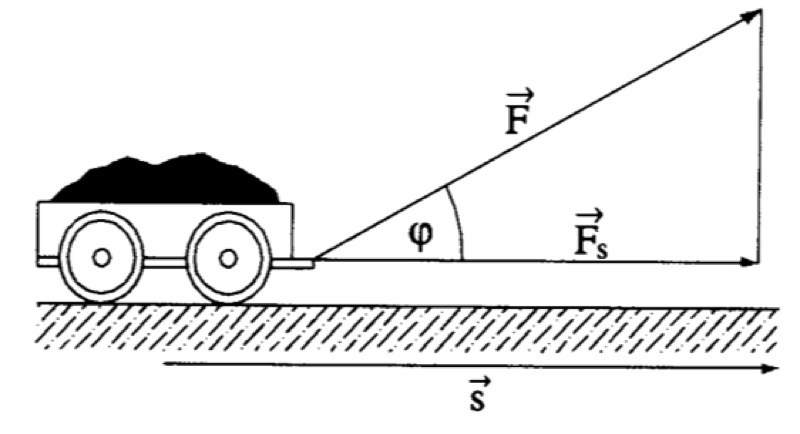
\includegraphics[width=0.49\textwidth]{pictures/arbeit}
\end{center}
\caption{Arbeit ist \glqq Kraft mal Weg\grqq}
\end{figure}

Benutzt man $F_s = F\cdot\cos\varphi$, so erhält man für die Arbeit
$$W = \vec{F_s}\cdot\vec{s} = F\cdot s \cdot \cos \varphi$$
Merkwürdig ist, dass die Verknüpfung zweier vektorieller Grässen (Kraft, Weg) eine skalare Grösse (Arbeit) ergibt. Ferner bemerken wir, dass die Länge von $\vec{F_s}$ vom Winkel $\varphi$ abhängt.

\section{Zerlegung eines Vektors}
Die Zerlegung eines beliebigen Ortsvektors nach den Basisvektoren $\vec{e}_x$ und $\vec{e}_y$ im rechtwinkligen Koordinatensystem ist ein Spezialfall eines allgemeineren Sachverhalts. Insbesondere bei physikalischen Problemen muss man oft eine Kraft in zwei Teilkräfte, deren Richtungen vorgegeben sind, zerlegen.

\begin{bsp}
\ \\[-4ex]
\begin{itemize}
\item Die Lampe einer Strassenbeleuchtung hängt an zwei Spannseilen. Die Gewichtskraft der Lampe wird in zwei Teilkräfte mit vorgeschriebenen Richtungen zerlegt.
\item Eine Kugel mit der Gewichtskraft $\vec{F_G}$ bindet sich auf einer schiefen Ebene mit Neigungswinkel $\alpha$. $\vec{F_G}$ lässt sich in die beiden Teilkräfte Hangabtriebskraft $\vec{F_H}$ und Normalkraft $\vec{F_N}$ zerlegen.
\end{itemize}
\end{bsp}

\clearpage

\section{Realistische Darstellungen mit dem Computer}
Wer kennt sie nicht, die Computergraphiken und -animationen in den Videoclips, in der Werbung, in kommerziellen und wissenschaftlichen Filmen, \dots?

\begin{itemize}
\item In einem Werbespot der Firma General Motors wird ein Sportwagen vom Typ Pontiac Fiero Bauteil für Bauteil über den Wolken montiert.
\item Für das Weltraum-Epos \glqq The Last Starfighter\grqq\ wurden im Computer --- ohne Modelle oder Zeichentrick-Vorlagen --- 27 Minuten Schlachtgetümmel und Sternreisen komponiert.
\item Die Digital Effects Studios in New York bauten im Computer einen Strassenzug Manhattans der 30er Jahre nach, in dem der Betrachter mit naturgetreu wechselnden Perspektiven zwischen Wolkenkratzern wandeln kann.
\item Am MIT wurde ein Computer-Trickfilm entwickelt, in dem ein nahezu lichtschnelles Raumschiff den Studenten die Tücken relativistischer Raumfahrt demonstriert.
\end{itemize}

Um wirklichkeitsgetreue Abbildungen zu erhalten, muss man die verschiedensten Dinge beachten wie zum Beispiel die Richtung des einfallenden Lichts, die Ober\-flä\-chen\-be\-schaf\-fen\-heit der darzustellenden Körper, deren Licht\-durch\-läs\-sig\-keit etc. In Wirklichkeit sind sehr wenige Flächen einfarbig. Oft beeinflussen Schattierungen, Spiegelbilder und durchscheinende Bilder das Ergebnis. Mit einfachen und komplizierten Algorithmen kann man heute schon sehr realistische Bilder erstellen. Im folgenden Abschnitt wird gezeigt, wie eine Tiefenwirkung durch die verschiedenen Be\-gren\-zungs\-flächen eines Körpers mit einer einfachen Idee erzeugt werden kann.

\begin{figure}
\begin{center}
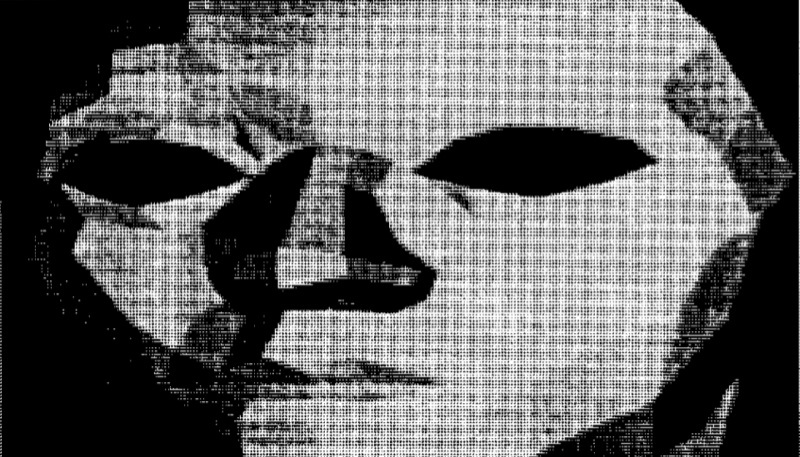
\includegraphics[width=0.7\textwidth]{pictures/pcgrafik}
\end{center}
\caption{Polygonmodell eines Kopfs}
\end{figure}

Wir gehen davon aus, dass der darzustellende Körper von einer Lichtquelle, die sich der Einfachheit halber im Unendlichen befindet, beleuchtet wird. Die Lichtstrahlen treffen auf die verschiedenen Begrenzungsflächen des Körpers auf und werden nach dem Reflexionsgesetz (Einfallswinkel=Ausfallswinkel) reflektiert.

\begin{figure}
\begin{center}
\definecolor{qqwuqq}{rgb}{0,0.39,0}
\definecolor{zzttqq}{rgb}{0.6,0.2,0}
\scalebox{0.8}{
\begin{tikzpicture}[line cap=round,line join=round,>=triangle 45,x=0.8cm,y=1.0cm]
\clip(-4.3,-0.72) rectangle (4.28,6.3);
\fill[color=zzttqq,fill=zzttqq,fill opacity=0.1] (-3.96,4.32) -- (-3,5) -- (0.72,-0.02) -- (-0.68,0) -- cycle;
\draw [shift={(-1.28,2.68)},color=qqwuqq,fill=qqwuqq,fill opacity=0.05] (0,0) -- (35.2:2) arc (35.2:51.25:2) -- cycle;
\draw [shift={(-1.28,2.68)},color=qqwuqq,fill=qqwuqq,fill opacity=0.05] (0,0) -- (20.87:2) arc (20.87:35.2:2) -- cycle;
\draw [color=zzttqq] (-3.96,4.32)-- (-3,5);
\draw [color=zzttqq] (-3,5)-- (0.72,-0.02);
\draw [color=zzttqq] (0.72,-0.02)-- (-0.68,0);
\draw (-1.28,2.68)-- (2.86,5.6);
\draw (-1.28,2.68)-- (1.4,6.02);
\draw (-1.28,2.68)-- (3.18,4.38);
\draw [->] (1.4,6.02) -- (0.02,4.3);
\draw [->] (-1.28,2.68) -- (0.8,3.47);
\draw[color=qqwuqq] (0,3.8) node {$\varphi$};
\draw[color=qqwuqq] (0.3,3.5) node {$\varphi$};
\end{tikzpicture}
}
\end{center}
\caption{Lichtreflexion an glatter Oberfläche}
\end{figure}

Man nimmt nun an, dass die Helligkeit einer Fläche nur durch den Einfallswinkel $\varphi$ bestimmt wird. In der Informatik benutzt man die \emph{Lambert'sche Regel}, die besagt, dass der Anteil des jeweils reflektierten Lichts gleich dem Cosinus des Einfallswinkels $\varphi$ ist.
Wenn $L$ die Intensität der Lichtquelle ist, so berechnet sich die Helligkeit $H$ der darzustellenden Fläche durch
$$H(\varphi)=k\cdot L\cdot\cos(\varphi)$$
wobei $k$ eine Materialkonstante ist. $k$ nimmt Werte zwischen $0$ und $1$ an und gibt den Prozentsatz des reflektierten Lichts an.

Mit Hilfe dieser einfachen Methode kann man mit verhältnismässig wenig Rechenaufwand schon erstaunlich gute Bilder erstellen.

\clearpage

\section{Das Drehmoment}

\begin{figure}[ht]
\begin{center}
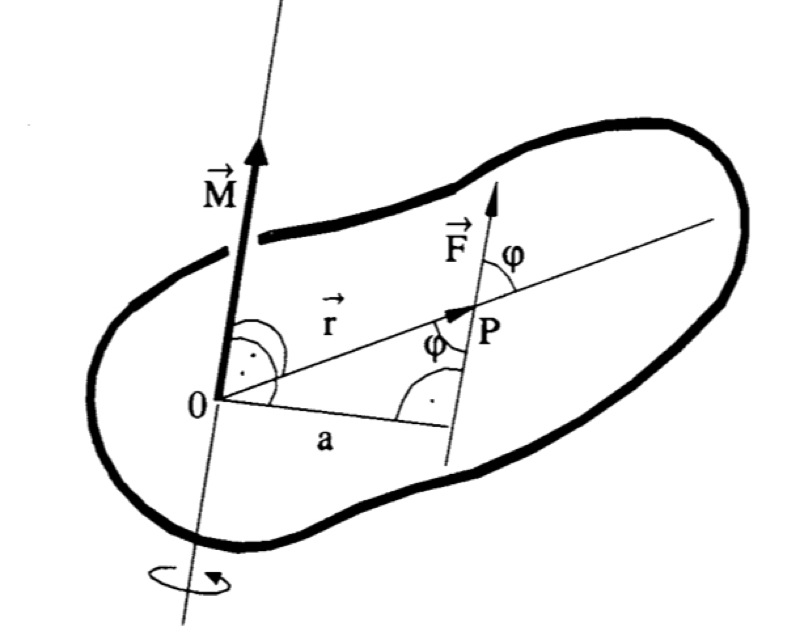
\includegraphics[width=5cm]{pictures/vprodukt}
\end{center}
\caption{Drehmoment $\vec{M}$}\label{abb:vektorprod}
\end{figure}

Auf den Körper wirke im Punkt $P$ eine Kraft $\vec{F}$ wie in Abbildung \ref{abb:vektorprod} auf Seite \pageref{abb:vektorprod} skizziert. Für die Berechnung des Drehmoments $M$ benötigt man nicht die Entfernung $r =\overline{OP}$, sondern den Abstand $a =r\cdot\sin\varphi$ der Wirkungslinie der Kraft vom Drehpunkt $O$:
$$M =a\cdot F =r\cdot F\cdot \sin\varphi$$

Physikalische Experimente zeigen:
\begin{itemize}
\item die Drehachse steht senkrecht zur Ebene, die durch
$\vec{r}$ und $\vec{F}$ aufgespannt wird,
\item die Drehrichtung wird durch $\vec{r}$ und $\vec{F}$ so bestimmt,
dass ein rechtshändiges System vorliegt ($\vec{r}$: Daumen,
$\vec{F}$: Zeigefinger, Drehrichtung: Mittelfinger der rechten Hand).
\end{itemize}
Man schreibt dafür:
$$\vec{M}=\vec{r}\times\vec{F}$$
(lies: \glqq $r$ Kreuz $F$\grqq)

\begin{bsp}
Eine nützliche Anwendung zeigt sich in der Elektrotechnik zur Bestimmung der Richtung der Lorentzkraft. Es gilt nämlich
$$\vec{F}=Q\cdot(\vec{v}\times\vec{B}),$$
wobei $Q$ für die Ladung, $\vec{v}$ für die Geschwindigkeit der Ladung und $\vec{B}$ für das Magnetfeld steht.
\begin{figure}
\begin{center}
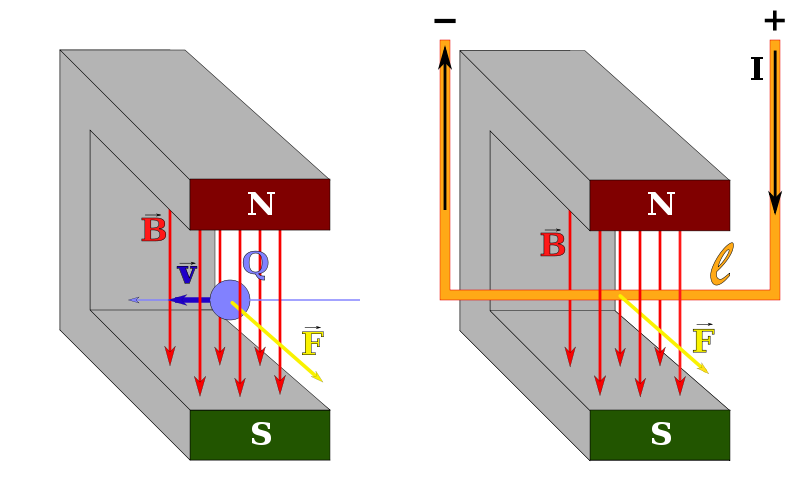
\includegraphics[width=0.4\textwidth]{pictures/lorentz.png}
\caption{Lorentzkraft $\vec{F}$}
\end{center}
\end{figure}
Der ausgestreckte rechte Zeigefinger folgt der technischen Stromrichtung, also der Bewegungsrichtung von positiv geladenen Ladungsträgern bzw. der entgegengesetzten Bewegungsrichtung negativer Ladungsträger.
Der ausgestreckte rechte Mittelfinger folgt der Richtung der Magnetfeldlinien, also der Richtung, in die sich der Nordpol eines Probemagneten ausrichtet.
Der rechte Daumen zeigt nun in die Wirkungsrichtung der Lorentzkraft.
\end{bsp}

\cleardoublepage

\listoffigures

\end{document}
